% Date : April 1, 2020
% Author : 
% Subhankar Mishra
% School of Computer Sciences 
% NISER
% \documentclass{book}
\documentclass[12pt,a4paper]{report}
\setlength{\oddsidemargin}{0.25in}
\setlength{\evensidemargin}{0.15in}
\setlength{\topmargin}{0.3in}
\setlength{\textwidth}{6.0in}
\setlength{\textheight}{8.5in}
\usepackage{amsmath,amssymb}
\usepackage{mathptmx}
\usepackage[linguistics]{forest}
\usepackage{mathptmx}
\usepackage[colorlinks]{hyperref}
\usepackage{epigraph}
\usepackage{algpseudocode}
\usepackage{algorithm}
\usepackage{graphicx}
\usepackage{caption}
\usepackage{subcaption}
% \usepackage{subfig}
% \usepackage{feynman}
\usepackage[T1]{fontenc}
\usepackage[utf8]{inputenc}
\usepackage{graphics}
\usepackage{lscape,graphicx}
\usepackage{amsfonts}
\usepackage{longtable}
\usepackage{epsfig}
\usepackage{float}
\usepackage{rotating}
\usepackage{caption}
\usepackage{listings}
\usepackage{mwe} % for blindtext and example-image-a in example
\usepackage{wrapfig}
\usepackage{lipsum}
\usepackage{fancyhdr}
% \usepackage{movie15}
\usepackage{hyperref}
\usepackage{graphicx}
\usepackage{epstopdf}
\epstopdfDeclareGraphicsRule{.gif}{png}{.png}{convert gif:#1 png:\OutputFile}
\AppendGraphicsExtensions{.gif}
\usepackage{lineno}
\usepackage{tikz-qtree}
\usepackage{biblatex}
\bibliography{test.bib}
\setlength{\headheight}{15pt}
\usepackage[titletoc]{appendix}
\usepackage[english]{babel}
\addto{\captionsenglish}{\renewcommand{\bibname}{References}}

\usepackage{titlesec}
\titlespacing*{\chapter}{0pt}{0pt}{0pt}
\titleformat{\chapter}[display]{\normalfont\huge\bfseries}{\chaptertitlename\ \thechapter}{20pt}{\Huge}

%%%%%%%%%%%%%%%%%%%%%%%%%%%%%%%%%%%%%%%%%%
%%%  macro for margin change
\newenvironment{changemargin}[2]{%
\begin{list}{}{%
%\setlength{\topsep}{0pt}%
\setlength{\leftmargin}{#1}%
\setlength{\rightmargin}{#2}%
%\setlength{\listparindent}{\parindent}%
%\setlength{\itemindent}{\parindent}%
%\setlength{\parsep}{\parskip}%
}%
\item[]}{\end{list}}
%%%%%%%%%%%%%%%%%%%%%%%%%%%%%%%%%%%%%%%%%%

\begin{document}
\begin{changemargin}{0cm}{0cm}
\thispagestyle{empty}
\baselineskip25pt
\begin{center}
{\Large {\bf Application of Machine Learning Techniques to Separate Resonance Particles From Background Processes}}\\
\end{center}

\vfill
% \baselineskip15pt
\begin{center}
{\textbf{ 9th-semester report \\Submitted}} \\
% in Partial Fulfilment of the Requirements \\
% for the Degree of \
% \vskip .30\baselineskip
% {\large{\bf MASTER OF SCIENCE}}
\end{center}
\baselineskip25pt

\vfill
\begin{center} {\bf {\em by}} \\
{\large{\bf SHIVAM RAJ}\\
1711127}\\


{{ \textit{ Supervised by:} }}\\
{\large{\bf Dr. Prolay Kr. Mal}}\\
\end{center}

\vfill
\begin{center}
\begin{figure}[h!]
\centering
\includegraphics[scale=0.5]{NISER.png}
% Reference for the Logo: Student Forms | NISER https://www.niser.ac.in/forms/academic/LaTexTemplate_MScThesis.zip
\end{figure}
 {\bf {\em to the }} \\
{\bf {\large School of Physical sciences}} \\
{\bf {\large National Institute of Science Education and Research}} \\
{\bf Bhubaneswar, India} \\
{\bf \today} 
\end{center}
\end{changemargin}



\pagenumbering{roman}
\baselineskip=20pt

% \begin{center}
% {\large {\bf DEDICATION (OPTIONAL)}} 
% \end{center}


% \include{declaration}
%\include{stat}
%\include{cert1}
\begin{center}
{\bf ACKNOWLEDGEMENTS}
\end{center}

I would like to express my deep gratitude towards all those people without whom this project would never have been completed. I want to give special appreciation to my supervisor, Dr. Prolay Kr. Mal, to provide me with the opportunity to work on this exciting work. Also, I also want to thank my supervisor for his enthusiasm, support, encouragement, and patience, which help me to complete this project.\\

Furthermore, I would like to express special gratitude to Prafulla Saha, without whose assistance this work remains uncompleted.  I also want to thank Chandiprashad Kar for his assistance and a healthy discussion over the doubts in the course of this project. Throughout this project, these people help me to clarify the problem and make it simpler for me to understand the reasoning behind the processes. I also want to thank other lab members, Aloke Kr. Das, Priyanka Sadangi, Lipsarani Panda, and other members for making a wonderful lab environment.\\

I also want to thank my friend, parents, and family for the patience and sacrifices they made during all this time.


\begin{center}
{\large {\bf  ABSTRACT }}\\
\textit{For extracting  signals, which are in small cross section compared to the large cross section of the background processes has been helped by the introduction of machine learning (ML) techniques for  classification purposes. Classification algorithms in machine learning is a type of supervised learning where the outputs are constrained only to a limited set of values or classes such as signals or backgrounds. A typical example would be the Higgs analysis. In this report, the classification of the produced resonance particles from p$\Bar{p}$ collision at Large Hadron Collider(LHC) is presented using machine learning technique trained with deep neural network(DNN). All the neural network training was done using Keras, TensorFlow, and Matplotlib in a Jupyter notebook. We will investigate all the challenges in the application of these novel analysis techniques in this report. This report concludes with a discussion of differences in the outcome of binary and multi-classification using DNN. 
}

% The Main Goal: To build a DNN to differentiate between signal and background events in an CMS data set
\end{center}  


    


\clearpage
\fancyfoot{}      % Delete current footer settings

\pagestyle{fancyplain}
 \renewcommand{\chaptermark}[1]{\markboth{\thechapter\ #1}{\thechapter\ #1}} % remember chapter title
 \lhead[\fancyplain{}{}]{\fancyplain{}{}}
 \rhead[\fancyplain{}{}]{\fancyplain{}{\em\leftmark }}
 \renewcommand{\headrulewidth}{0.3pt}
 \cfoot{\rm\thepage} % page number

\baselineskip=12pt
\tableofcontents
\clearpage
\listoffigures
\clearpage
\listoftables 
\clearpage
\pagenumbering{arabic}
\baselineskip=24pt
\chapter{\label{intro}Introduction}
% \linenumbers
% Managing the large amount of data from the Large Hadron Collider (LHC) collisions is a major challenge for CMS physicists.As the detector produces millions of data per second, precisely around 500 tetrabytes of data per second. After filtering of the collision events online within a fraction of a second, many bytes of data are saved offline for further analysis. Since, there is a plan to increase the luminosity of the LHC (upto 5 times of the present), it would be very challenging in the future. To meet this challenge, CMS physicists are using state-of-the-art machine learning methods at every stage of the data processing, to improve the experiment. From real-time filtering to offline data analysis, they are using machine learning to improve physics performance, accelerate computations, improve data quality, and optimize searches for new physics signatures.\\

The machine learning algorithms, which is general and not task-specific, are modeled towards improving the  performance on some given task by training on more and more data\cite{1-5}. The training of the machine depends on the past data. The data split in training, validation set and test subsets. The first two are often combined together, where a different chunk of the data is used at each training step to estimate the predictive power of a model. The ultimate goal of the model is a generalization of its ability as to how well it performs over unseen data ot the test data,  which can be real or future data. To avoid the problem of overfitting in the model, in ML approximate solutions are preferred: where the goal is to learn all the essential features of the data and further generalize the model[\cite{4}]. \\


This project report is based on case studies using simulated data for the CMS detector. Our primary objective is to make such a model search for the rare processes of the resonance particle such as Tprime using machine learning techniques. Tprime(T') is one vector-like quark, which decays into a standard model(SM) top quark and a Higgs boson with decaying into two photons.  \cite{12}.


% Discuss about T'
% With the increasing complexity of events in high energy physics, the importance
% of multivariate analysis for LHC has been recognized before the start of data taking.
% The main motivation was to go beyond the traditional methods for event selection by applying series of cuts on individual variables, and be able to use correlations
% and more intricate patterns in the multidimensional data.\\

Compact Muon Solenoid (or CMS) detector located at one of these four collision points of the LHC[[\cite{15-20}]. It is designed to observe any new physics phenomena that the LHC might reveal. CMS acts as a giant, high-speed camera, taking 3D "photographs" of particle collisions from all directions up to 40 million times per second. It is 15m in diameter. The central device around which the experiment is built is its magnet, which carries a total magnetic field of 4 Tesla(4T). The Charged particle trajectories after the collision are measured by the silicon pixel and strip sub-detectors, covering 0 <$\phi$ <2$\pi$ in azimuth and $|\eta|$ < 2.5, where the pseudo rapidity $\eta$ is defined as 
 \begin{equation*}
     \eta = -ln[\tan \theta/2],
 \end{equation*}
 
 where $\theta$ is the polar angle of trajectory of the particle with counterclockwise beam direction. Within the field
volume, the silicon detectors are surrounded by a crystal electromagnetic calorimeter and a brass/scintillator hadron calorimeter that provides high resolution energy measurement of photons, electrons, and hadronic jets.\\

Machine learning has very vast applications in High energy physics(HEP). Earlier, a decision function often used as decision tree. These decision trees also behave like a natural tree-like model to make the decision, starting at the root, further climbing up the branches and then reaching to the leaves, where leaves behave like decision. For classification problem, each leaf represents our decisions to assign the data into classes, whether it is binary or multiclass classifications\cite{7-8}. The most widely used machine learning techniques in HEP are boosted decision trees(BDT), XgBoosts, etc \dots\\



Neural networks, also known as artificial neural networks(ANN), are structures inspired by the human brain and also mimic the connectivity of biological signals to one another. The neurons and synapses have been replaced with connected layers of
nodes ( neurons) and edges. A node takes inputs as real numbers (a weighted sum of the connected outputs from the previous layer) and performs a non-linear transformation to form its output. These non-linear transformation functions are known as the \textbf{activation function}. Typical activation functions are: sigmoid (logistic) and tanh where the output is limited below  % [\url{https://www.phys.ufl.edu/~avery/ivdgl/itr2001/proposal_all.pdf}]  
for any input values, and the rectified linear unit ReLU (max(0, x) or the positive part of the argument.\\
Each  neural network consists of at least an input, an output, and one or more hidden layers. This is part of Deep learning. We represent deep NN as DNN. The learning can be supervised depending on pairs of inputs with known outputs for training, or unsupervised, or semi-supervised. A cost or loss function measures the “distance” between the current and the desired outcomes, where our main goal is to make a loss as little as possible to train the model. Classical optimization aims to minimize the cost function on the available (training) data, with or main goal in ML is to generalize, or minimize the cost best, on the unseen or the test data. At each step, the weights for all the edges can be adjusted by backpropagation based on the differentiation chain rule to reduce the cost function by small amounts. This is the stochastic gradient descent (SGD)\cite{4}.\\

Here, in this project report, we will discuss all the basic concepts related to machine learning in detail. The outline of this report are as follows: \autoref{Method}  discusses the basic concepts related to machine learning and deep learning(DNN), and further about the simulated data sample used for the separation of signal and background is discussed in \autoref{d}. We will discuss the results and outputs obtained after DNN training in \autoref{results}, and finally, conclude this report with the conclusion in \autoref{summary}. 


% file:///home/sraj/Documents/M.sc._Project/Date_WISE/nov_21/9_nov/Introduction%20to%20Machine%20Learning.html
\setcounter{equation}{0}
\setcounter{table}{0}
\setcounter{figure}{0}
%\baselineskip 24pt


    




% \chapter{\label{The CMS detector}The CMS detector}
The 27-km Large Hadron Collider (LHC) is the largest and most powerful particle accelerator ever built. It accelerates protons to nearly the velocity of light -- in clockwise and anti-clockwise directions -- and then collides them at four separate locations around its ring as shown in the \autoref{fig:my_label_LHC}. At these points, the energy of the particle collisions gets transformed into mass, spraying particles in all directions (\url{https://cms.cern/detector}).
% This will help us answer questions such as: "what is the Universe really made of and what forces act within it?" and "what gives everything substance?" Such research increases our basic understanding and may also spark new technologies that change the world we live in.\\
The Compact Muon Solenoid (or CMS) detector located at one of these four collision points. It is designed to observe any new physics phenomena that the LHC might reveal.CMS acts as a giant, high-speed camera, taking 3D “photographs” of particle collisions from all directions up to 40 million times per second. Although most of the particles produced in the collisions are “unstable” and short-lived, they transform rapidly into stable particles which can be detected by CMS.\\
 CMS is 15 meters in diameter. The CMS magnet is the central device around which the experiment is built, with a 4 Tesla magnetic field that is nearly $10^6$ times stronger than the Earth’s.(\url{https://cms.cern/detector/bending-particles})
 \begin{figure}[H]
     \centering
     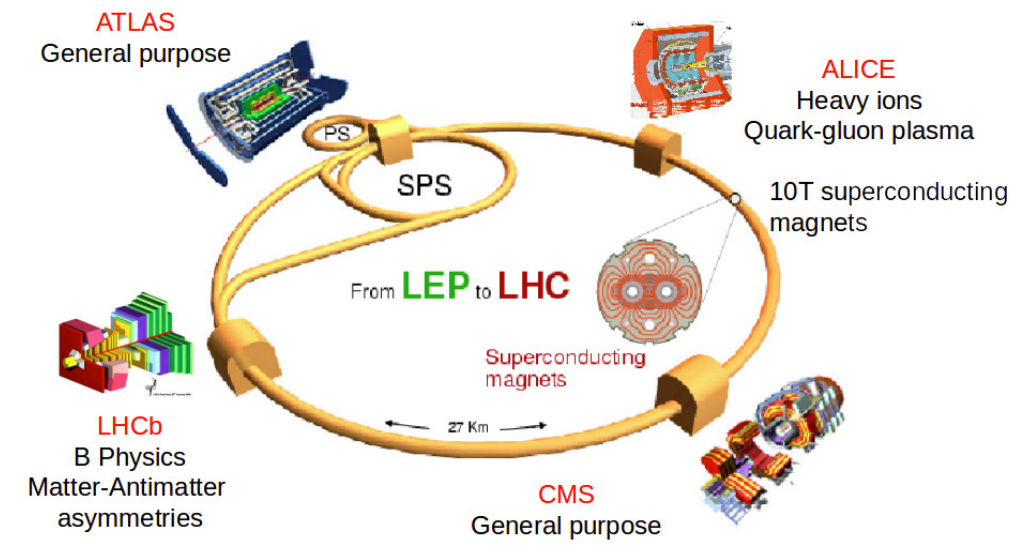
\includegraphics[scale=0.3]{14__ml.png}
     \caption{LHC}
     \label{fig:my_label_LHC}
 \end{figure}
As we know, higher the energy of the particle, the greater the amount of material needed to track. Similarly, to measure the momentum of a particle we track its path with the help of magnetic field, as greater the momentum the less it bends within it.
\url{https://cms.cern/detector}\\



The more momentum a particle has the less possibility of its path may get curved by the magnetic field, so tracing its path gives a measure of momentum of the particles. The tracker and calorimeter detectors (ECAL and HCAL) fit snugly inside the magnet coil whilst the muon detectors are inserted with a 12-sided iron structure that surrounds the magnet coils and contains and guides the field(as can be seen from the \autoref{fig:my_label_detect}).[\url{https://cms.cern/detector/bending-particles}]
The main function of CMS:
\begin{itemize}
    \item Bending Particles
    \item Identifying tracks
    \item Measuring energy
    \item Detecting muons
\end{itemize}
There are many other use such as medical imagining and etc.\\

 CMS consists of layers of detector material that exploit the different properties of particles to catch and measure the energy or momentum of each one. New particles discovered in CMS will be typically unstable and rapidly transform into a cascade of lighter, more stable and better-understood particles

\begin{figure}[h]
    \centering
    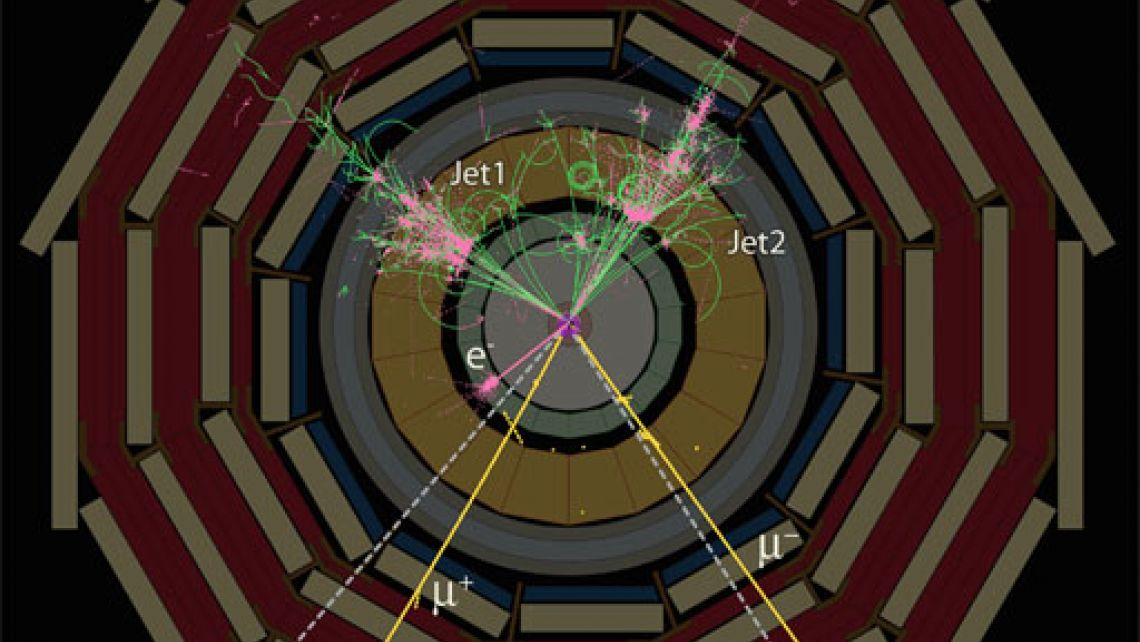
\includegraphics[scale=0.3]{Figures/SusyAny.jpg}
    \caption{This event shows the production of a supersymmetric particle. The decay of the particle is such that every single layer of CMS is needed to detect the full range of emerging particles: electrons, muons, neutrinos and jets, produced by quarks.[Source: \url{https://cms.cern/news/how-cms-detects-particles}]}
    \label{fig:my_label}
\end{figure}


% \includemovie{1cm}{1cm}{Figures/detectoroverview.gif}
% \includegraphics{Figures/detectoroverview.gif}
A particle which emerges from the collision, travel outwards will first encounter the tracking system, made of silicon pixels and silicon strip detectors. This pixels and strip detectors act as a camera. These accurately measure the positions of passing charged particles and allowing physicists to reconstruct their tracks. Charged particles follow spiraling paths in the CMS magnetic field and the curvature of their paths reveal their momenta.[\url{https://cms.cern/news/how-cms-detects-particles}]\\
The energies of the emerged particles will be measured in the next layer of the detector, the so-called calorimeters. Electrons, photons and jets (sprays of particles produced by quarks) will all be stopped by the calorimeters, allowing their energy to be measured.The first calorimeter layer is designed to measure the energies of electrons and photons with great precision. Since these particles interact electromagnetically, it is called an electromagnetic calorimeter (ECAL).[\url{https://cms.cern/detector/measuring-energy}]\\
Particles that interact by the strong force, hadrons, deposit most of their energy in the subsequwnt layer, the hadronic calorimeter (HCAL). The only known particles to penetrate beyond the HCAL are muons and weakly interacting particles such as neutrinos. Muons are charged particles, which are then tracked further in muon chamber detectors. Their momenta are also measured from the bending of paths in the CMS magnetic field. Neutrinos, however, are neutral and since they hardly interact at all they will escape detection.By adding up the momenta of all the detected particles, and assigning the missing momentum to the neutrinos, we can tell where these particles were.\\

% \section{TRIGGERING AND DATA ACQUISITION}
We need a "trigger" to select the potentially interesting events (such as Higgs particle) from larger amount of data produces after collision of proton-proton interaction. These trigger helps to reduce the rate to just a few hundred “events” per second, which can be read out and stored on computer disk for subsequent analysis. At the end, We are only left with only the collision events that might teach us something new about physics.[\url{https://cms.cern/detector/triggering-and-data-acquisition}]\\ 
% When CMS is performing at its peak, about one billion proton-proton interactions will take place every second inside the detector. There is no way that data from all these events could be read out, and even if they could, most would be less likely to reveal new phenomena; they might be low-energy glancing collisions for instance, rather than energetic, head-on interactions.We therefore need a “trigger” that can select the potentially interesting events, such as those which will produce the Higgs particle, and reduce the rate to just a few hundred “events” per second, which can be read out and stored on computer disk for subsequent analysis.\\

% However, with groups of protons colliding 40 million times per second there are only ever 25 nanoseconds (25 billionths of a second) before the next lot arrive. New waves of particles are being generated before those from the last event have even left the detector! The solution is to store the data in pipelines that can retain and process information from many interactions at the same time. To not confuse particles from two different events, the detectors must have very good time resolution and the signals from the millions of electronic channels must be synchronised so that they can all be identified as being from the same event.\\
% Level 1 of the trigger is an extremely fast and wholly automatic process that looks for simple signs of interesting physics, e.g. particles with a large amount of energy or in unusual combinations. This is like a reader simply scanning the headlines of a newspaper to see if anything catches their eye. This way we select the best 100,000 events or “issues” each second from the billion available. For the next test, the higher level trigger, we assimilate and synchronise information from different parts of the detector to recreate the entire event - like collating the different pages to form the full newspaper - and send it to a farm of more than 1000 standard computers.


% \url{https://cms.cern/detector/triggering-and-data-acquisition}


% \section{SILICON STRIPS}
% https://cms.cern/detector/identifying-tracks/silicon-strips
On the way out of the tracker, particles pass through ten layers of silicon strip detector of 130 centimeters.This tracker silicon strip detector consists of four inner barrel (TIB) layers assembled in shells with two inner endcaps (TID), each with three small discs. The outer barrel (TOB) consists of six concentric layers( as seen in \autoref{}). Finally two endcaps (TEC) close off the tracker. Each has silicon modules designed differently for its place within the detector. This part of the tracker contains 15,200 highly sensitive modules with a total of 10 million detector strips read by 80,000 microelectronic chips. Each module consists of three elements: sensors, mechanical support structure and electronics. These silicon are very suited to receive many particles in a small space due to their fast response and good spatial resolution. The small amount of charge generated after knocking of electron from atoms get amplified by APV25 chips, allows us to reconstruct its path.


\begin{figure}[H]
    \centering
    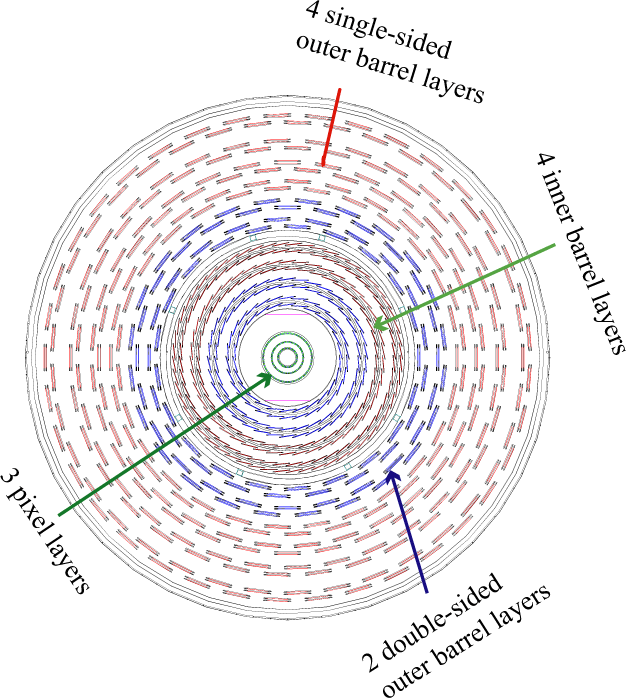
\includegraphics[scale=0.5]{Barrel.png}
    \caption{CMS Tracker layer shown in perpendicular to the beam[Source:\url{https://cms.cern/detector/identifying-tracks/silicon-strips}]}
    \label{fig:my_label}
\end{figure}


% After the pixels and on their way out of the tracker, particles pass through ten layers of silicon strip detectors, reaching out to a radius of 130 centimetres.
% The tracker silicon strip detector consists of four inner barrel (TIB) layers assembled in shells with two inner endcaps (TID), each composed of three small discs. The outer barrel (TOB) consists of six concentric layers. Finally two endcaps (TEC) close off the tracker. Each has silicon modules designed differently for its place within the detector. This part of the tracker contains 15,200 highly sensitive modules with a total of 10 million detector strips read by 80,000.  Each module consists of three elements: a set of sensors, its mechanical support structure and readout electronics. \\
% Silicon sensors are highly suited to receive many particles in a small space due to their fast response and good spatial resolution. microelectronic chips. Each module consists of three elements: a set of sensors, its mechanical support structure and readout electronics. \\
% Silicon sensors are highly suited to receive many particles in a small space due to their fast response and good spatial resolution. The silicon detectors work in much the same way as the pixels: as a charged particle crosses the material it knocks electron from atoms and within the applied electric field these move giving a very small pulse of current lasting a few nanoseconds. This small amount of charge is then amplified by APV25 chips, giving us “hits” when a particle passes, allowing us to reconstruct its path.

% Due to the nature of their job, the tracker and its electronics are pummeled by radiation but they are designed to withstand it. To minimise disorder in the silicon this part of the detector is kept at -20oC, to “freeze” any damage and prevent it from perpetuating.

% The charge on each microstrip is read out and amplified by an Analogue Pipeline Voltage (APV25) chip. Four or six such chips are housed within a “hybrid”, which also contains electronics to monitor key sensor information, such as temperature, and provide timing information in order to match “hits” with collisions. The APV25 stores the signals in a memory for several microseconds and then processes them before sending to a laser to be converted into infrared pulses. These are then transmitted over a 100m fibre optic cable for analysis in a radiation-free environment. The tracker uses 40,000 such fibre optic links providing a low power, lightweight way of transporting the signal. Much of the technology behind the tracker electronics came from innovation in collaboration with industry. \\
% \section{SILICON PIXELS}

% https://cms.cern/detector/identifying-tracks/silicon-pixels

% \section{TRACKING}
% https://cms.cern/detector/identifying-tracks

% The pixel detector, though about the size of a shoebox, contains 65 million pixels, allowing it to track the paths of particles emerging from the collision with extreme accuracy. Each layer is spilt into segments like tiny kitchen tiles, each a little silicon sensor, 100µm by 150µm, about two hairs widths. When a charged particle passes through it gives enough energy for electrons to be ejected from the silicon atoms, creating electron-hole pairs. Each pixel uses an electric current to collect these charges on the surface as a small electric signal. A electronic silicon chip, one for each tile is attached, using an almost microscopic spot of solder using the so-called bump bonding technique, which amplifies the signal.Knowing which pixels have been touched allows us to deduce the particle's trajectory. And because the detector is made of 2D tiles, rather than strips, and has a number of layers, we can create a three-dimensional picture. Because there are 65 million channels, the power for each pixel must be kept to a minimum. Even with each only generating around 50 microwatts, the total power output is around the same as the energy produced by a hot plate. So as not to overheat the detector, the pixels are mounted on cooling tubes.\\
% % \section{MEASURING ENERGY}
% https://cms.cern/detector/measuring-energy
The Electromagnetic Calorimeter (ECAL) is the inner layer of the two and measures the energy of electrons and photons by stopping them completely. Hadrons, which are composite particles made up of quarks and gluons, fly through the ECAL and are stopped by the outer layer called the Hadron Calorimeter (HCAL). Photodetectors that have been especially designed to work within the high magnetic field, are also glued onto the back of each of the crystals to detect the scintillation light and convert it to an electrical signal.
 
% \section{ENERGY OF ELECTRONS AND PHOTONS (ECAL)}
% https://cms.cern/detector/measuring-energy/energy-electrons-and-photons-ecal\\
% CMS must find the energies of emerging particles. Of particular interest are electrons and photons, because of their use in finding the Higgs boson and other new physics.

% The particles are measured using an electromagnetic calorimeter (ECAL). But to find them with the necessary precision in the very strict conditions of the LHC - a high magnetic field, high levels of radiation and only 25 nanoseconds between collisions - required very particular detector materials.\\ 
% Lead tungstate crystal is made primarily of metal and is heavier than stainless steel, but with a touch of oxygen in this crystalline form it is highly transparent and “ scintillates ” when electrons and photons pass through it. This means it produces light in proportion to the particle’s energy. These high-density crystals produce light in fast, short, well-defined photon bursts that allow for a precise, fast and fairly compact detector.

% Photodetectors that have been especially designed to work within the high magnetic field, are also glued onto the back of each of the crystals to detect the scintillation light and convert it to an electrical signal that is amplified and sent for analysis.

% The ECAL, made up of a barrel section and two ”endcaps”, forms a layer between the tracker and the HCAL. The cylindrical “barrel” consists of 61,200 crystals formed into 36 “supermodules”, each weighing around three tonnes and containing 1700 crystals. The flat ECAL endcaps seal off the barrel at either end and are made up of almost 15,000 further crystals.

% For extra spatial precision, the ECAL also contains Preshower detectors that sit in front of the endcaps. These allow CMS to distinguish between single high-energy photons (often signs of exciting physics) and the less interesting close pairs of low-energy photons.
% The CMS ECAL…

% crystals each weigh 1.5kg but with a volume roughly equal to that of a small coffee cup,
% contains nearly 80,000 such crystals, each of which took two days to grow.

% https://cms.cern/detector/measuring-energy/energy-hadrons-hcal\\

% https://cms.cern/detector/detecting-muons\\
% https://cms.cern/detector/computing-grid\\
A huge amount of data, obtained from CMS that must be analysed, and to meet this challenge, the LHC employs a novel computing system, a distributed computing and data storage infrastructure called the Worldwide LHC Computing Grid (WLCG). In ‘The Grid’, tens of thousands of standard PCs collaborate worldwide to have much more processing capacity than could be achieved by a single supercomputer, giving access to data to thousands of scientists all over the world.\url{https://cms.cern/detector/computing-grid}

% The “Tier 0” centre at CERN first reconstructs the full collision events and analysts start to look for patterns; but the data has a long way to go yet. Once CERN has made a primary backup of the data it is then sent to large “Tier 1” computer centres in seven locations around the world: in France, Germany, Italy, Spain, Taiwan, the UK and the US. Here events are reconstructed again, using information from the experiment to improve calculations using refined calibration constants.

% Tier 1 starts to interpret and make sense of the particle events and collate the results to see patterns emerging. Meanwhile each sends the most complex events to a number of “Tier 2” facilities, which total around 40, for further specific analysis tasks. In this way information braches out from each tier across the world so that, on a local level.
% , physicists and students whether in Rio de Janeiro or Oxford, can study CMS data from their own computer, updated on a regular basis by the LHC Computing Grid.
 Charged particle trajectories are measured by the silicon pixel and strip sub detectors, covering 0 <$\phi$ <2$\pi$ in azimuth and $|\eta|$ < 2.5, where the pseudo rapidity $\eta$ is defined as 
 \begin{equation*}
     \eta = -ln[\tan \theta/2],
 \end{equation*}
 
 with $\theta$ being the polar angle of the trajectory of the particle with respect to the counterclockwise-beam direction. Within the field
volume, the silicon detectors are surrounded by a crystal electromagnetic calorimeter and a brass/scintillator hadron calorimeter that provide high resolution energy measurement of photons, electrons and hadronic jets.

\setcounter{equation}{0}
\setcounter{table}{0}
\setcounter{figure}{0}
%\baselineskip 24pt


    




\chapter{\label{Method}Machine Learning}
\epigraph{Machine Learning can be defined as the process of inducing intelligence into a system or machine without explicit programming}{-Andrew NG}
The machine learning (ML) subset of artificial intelligence (AI) allows computer applications to become more accurate by predicting outcomes without being explicitly programmed(not providing commands on each step).  The algorithms used by the machines depend on historical or past data as input to predict new outputs. We are surrounded by numerous applications of machine learning in our daily life such as image recognition software's, speech recognition(Voice search, voice dialing), Predictive analytics(Predicting whether a transaction is fraudulent or legitimate, Whether mail is spam or not), etc.

Machine learning is very important nowadays as it provides an overview of trends in customer behavior and operational business patterns, also supports the development of new products. The most common examples can be taken from today's leading tech companies, such as Facebook, Google, and car rental companies, Uber, which use machine learning as a central part of their operations. For handling a large amount of data, machine learning has always been an efficient method. This chapter discusses the basic concept of machine learning and how neural network functions, which are more efficient and productive compared to traditional workflow.[\cite{25-26}]


\section{Types of Machine Learning:}
There are four basic approaches for machine learning: supervised learning, unsupervised learning, semi-supervised learning, and reinforcement learning. The type of algorithm that will be used depends on what type of data they want to predict.
\subsection{Supervised Learning}
In this type of machine learning, we supply algorithms with labeled training datasets and define the variables that we want the algorithm to assess for correlations and the outputs. 
Both the input and the output of the algorithm have been already specified. Supervised machine learning requires getting trained with the algorithm on both labeled inputs and desired outputs. A simple example would be the classification of datasets.
\subsection{Unsupervised learning:}
This type of machine learning involves algorithms that train on unlabeled datasets. The algorithm scans through datasets looking for any meaningful connection without any human intervention. The data on which algorithms train as well as the predict the output is predetermined. For example, unsupervised learning is used for Google news categorization, visual perception tasks such as image recognition, anomaly detection, classifying customers, etc.

\subsection{Semi-supervised learning:}
This approach to machine learning involves a mix of both the previous types of the dataset; that is algorithm is trained upon the combination of the labeled and unlabeled dataset.  In this type of algorithm, the programmer just needs to cluster similar data using an unsupervised learning algorithm and further use the existing labeled data to label the rest of the unlabeled data. A few practical examples of this type of learning are speech analysis, internet content classifications, and protein sequence classification.


\subsection{Reinforcement learning: }
Data scientists usually use reinforcement learning to teach a machine to complete a multistep process( based on the rewarding behaviors/ or pushing the undesired one ) for which there is a clearly defined set of rules. In the reinforcement learning decision is dependent on the output of the previous input sequence, so we provide labels to sequences of dependent decisions. For example, chess games or a sitting cat, the cat will only get food when she starts to walk.\\

A brief summary of how machine learning consists can be summarized from this tree diagram,
% \textbf{Add examples to each of the learning}
\resizebox{\linewidth}{!}{%
\begin{center}
    \begin{forest}
  [Machine Learning
    [Supervised \\ Learning
     [Classification 
       [Binary \\ classification]
       [Multi \\classification]
     ]
     [Regression
       [Regression \\ modeling
         [\textit{Ensembling}]
       ]
     ]
    ]
    [Unsupervised \\ Learning
      [Clustering
      [K-means Clustering]
      ]
      [Anomaly detection
        % [V$'$
        %   [V
        %     [\textit{is}]
        %   ]
        %   [AP
        %     [Deg
        %       [\textit{extremely}]
        %     ]
        %     [A$'$
        %       [A
        %         [\textit{straightforward}]
        %       ]
        %       [CP
        %         [\textit{to wield}, roof]
        %       ]
        %     ]
        %   ]
        % ]
      ]
    ]
    [semi-supervised\\ learning
    ]
    [reinforcement \\learning
    ]
  ]
\end{forest}
\end{center}
}%

\section{Evaluating models}
In machine learning, the ultimate goal is to achieve models that generalize, i.e., that perform well on never-before-seen data, and overfitting is the central obstacle. To do this, splitting the available data is very crucial. Training, validation, and testing are the partitions  
needed, so during the training phase, the model trains with the training data and test with the validation data, and when the model is ready, it is tested one last time with the test data, briefly explained by \autoref{fig:my_label_09876} \\
\begin{figure}[H]
    \centering
    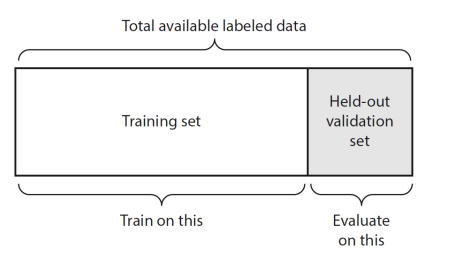
\includegraphics[scale=0.6]{ml__12.png}
    \caption{Splitting data to be used in the training phase. Image source: [Chollet, 2017]}
    \label{fig:my_label_09876}
\end{figure}
The reason why three (and not two) datasets are used is that tuning in the model configuration is required. The parameters that can be tuned in a machine learning model are called hyperparameters. Hyperparameter values can be changed to control the learning process. Meanwhile, the value of other parameters, like node weights, are derived by training and cannot be adjusted. Hyperparameter tuning is done with the feedback of the model performance in the validation data and further applied under an unseen test dataset. This is a basic approach for each machine learning model, and we will apply the same over the neural network model in the next section.

%%%%%%%%%%%%%%%%%%%%%%%%%%%%%%%%%%%%%%%%%%%%%%%%%%%%%%DNNNNNNNNNNNNNDNNNDNNNDNNNNDNNDNNNDNNDNDNNDNDNNDNDNNNDNNNNDNNNDNDNDNDNDNDNDNDNDNDNNDNDNDNDNNDND
\section{Deep Neural Network}
Machine learning works very efficiently on numerous problems but sometimes fails to excel in a few specific cases, which appears very easy for humans. For example, classifying an image as a cat or dog or distinguishing audio clips as a male or female voice,etc\dots The machine fails to identify this type of problem of image classification or video segregation and other unstructured data types, which are easy for us. There come to the idea of a deep neural network(DNN), where the idea is to mimic the human brain's biological process, which is composed of billions of neurons connected to each other and to adapt and learn new things\cite{23-25}. \\ 


A simplified version of Deep Neural Network can be represented as a hierarchical (layered) structure of neurons (compared with the neurons in the human brain) with connections to other neurons. These neurons pass a message or signal to other neurons based on the received input and form a complex network system that learns with some feedback mechanism. The following diagram(\autoref{fig:my_label_hu}) represents an 'N' layered Deep Neural Network.\\

\begin{figure}[H]
    \centering
    \includegraphics[scale=0.4]{1_ML_report.png}
    \caption{A Deep Neural Network with N hidden layers}
    \label{fig:my_label_hu}
\end{figure}
The input data is provided to the neurons into the first layer (not hidden), which subsequently provides an output to the neurons within the next layer and so on and finally provides the final output. These outputs might be a prediction such as Yes or No (just as we represent in probability). Each layer can consist of one or many neurons, and each of them will be computed with the help of a small function, i.e., activation function. The activation function takes the signal from the previous layers and passes it further to the next connected neurons. There is a threshold value corresponding to each activation function, where the output is passed when it is above the threshold value; else, it gets ignored. The connection between two neurons of successive layers always passes with an associated weight. \\
 
 The weights have a very important role to play in the correct prediction from the model. This weight defines the influence of the input on the output for each layer. We provide initial weight to the model randomly, but during the training, these weights get updated iteratively to learn to predict a suitable output.\\
 In a neural network, the initial weights would be provided by us as a random number, but during the model training, these weights are updated iteratively by themselves to learn to predict a correct output. The network also depends on the learning mechanism (optimizer), which helps the neural network to update its weights (that were randomly initialized) to a more suitable weight that aids in the correct prediction of the outcome.  To update its weight for the connections, the mathematical algorithm used is called backpropagation. The iteration of the process several times, with more and more data, helps the model to update its weights appropriately. By iterating the process several times, with the help of more data, the networks update the weights appropriately to create a system where the system can take a decision for predicting output based on rules which the model created for itself with the help of weights and connections\cite{22-23}.\\


Deep learning is efficient to work with a large amount of data which has made it popular in the last few years; a few of the popular choices for the frameworks of deep learning in python are:-\\
 \begin{itemize}
     \item Low-level frameworks 
         \begin{itemize}
             \item TensorFlow
             \item MxNet
             \item PyTorch
         \end{itemize}
      \item High-level frameworks
         \begin{itemize}
             \item Keras (uses TensorFlow as a backend)
              \item Gluon (uses mxnet as a backend)
         \end{itemize}
 \end{itemize}

Schematically, a neural network(unit, node) layer can be represented as in below \autoref{fig:my_label_3}. 
\begin{figure}[H]
    \centering
    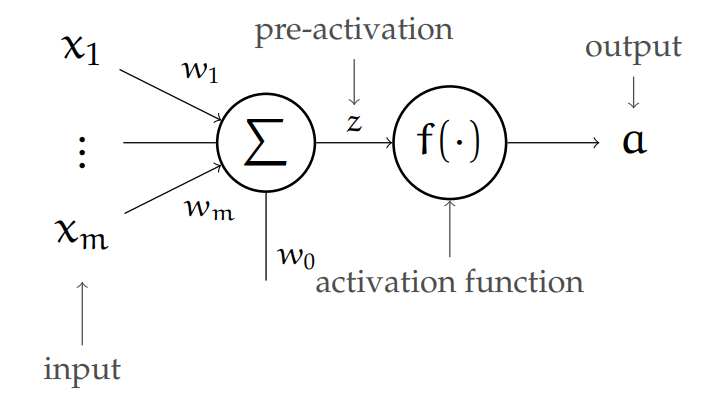
\includegraphics[scale =0.5]{Figures/ml__1.png}
    \caption{Basic structure of a neural network}
    \label{fig:my_label_3}
\end{figure}




The function representing the neural network can be expressed as:

\begin{equation}\label{eq:eq1}
a= f(z) = f(\sum_{j=1}^{j=m} x_jw_j +w_0) = f(w^T x+w_0)
\end{equation}
A non-linear function of an input vector x $\in \mathbb{R}^m$ note to a single output value  a $\in$R . It is parameterized by a vector of weights  $(w_1, w_2,....w_m)\in \mathbb{R}^m$  and an offset or threshold  $w_0\in \mathbb{R}^m$ . In order for the neuron to be non-linear, we also specify an activation function  $f:\mathbb{R} \to \mathbb{R}$ , which can be the f(x)=x(linear function), or can also be any other non linear function, such as ReLU, tanh, etc., which is differentiable. 
\\
Before thinking about a whole network,let us consider how to train a single unit. \\
Given a loss function L(guess, actual) and a dataset $\{(x^{(1)},y^{(1)}),.....,(x^{(n)},y^{(n)})\}$, we can do (stochastic) gradient descent, adjusting the weights w, $w_0$ to minimize the equation 

\begin{equation} \label{eq:eq2}
    J(W, W_0) = \sum_{i=1} ^n L(f(x^{(i)}:W),y^{(i)})
\end{equation}
where f is the output of our neural net for a given input.

% \textbf{Provide example here :linear logistic classifiers (LLC)
% with NLL loss and regressors with quadratic loss! The activation function for the LLC is
% f(x) = $\sigma$(x) and for linear regression it is simply f(x) = x. \\
% Just for a single neuron, imagine for some reason, that we decide to use activation function f(z) = $e^z$ and loss function $L(g, a) = (g-a)^2$. Derive a gradient descent update for w and $w_0$.}

%%%%%%%%%%%%%%%%%%DO from here%%%%%%%%%%%%%%%%%%%
\subsection{Networks}


Now, we’ll try to train the network with stacking multiple neurons together to form a network. A neural network in general takes input $x \in \mathbb{R}^m$ and generates an output $\alpha \in \mathbb{R}^n $.  It is constructed with the help of multiple neurons; the inputs of each neuron might be elements of x and/or outputs of other neurons. The outputs are generated by n output units.
Here, for the training of data, we will only consider feed-forward networks. In a feed-forward network, we can think of the network as defining a function-call graph that is acyclic. For the simplicity in software and analysis, we usually organize networks into layers. A \textbf{layer} can be defined as a group of neurons which are connected to each other parallelly (as in \autoref{fig:my_label_hu}): The input of a hidden layer depends on the output of previous layer(hidden or input layer); and the output from the layers are input to the neurons in the subsequent next layer. We will start to describe about the model with a single layer and further go on to the case of multiple layers.

\subsubsection{Single-layer}
A layer is a set of units that, as we have just described, are not connected to each other. The
layer is called fully connected if, as in the diagram below, the inputs to each unit in the layer
are the same. A layer has input x $\in \mathbb{R}^m$ and output (also known as activation) $\alpha \in \mathbb{R}^n$
\begin{figure}[H]
    \centering
    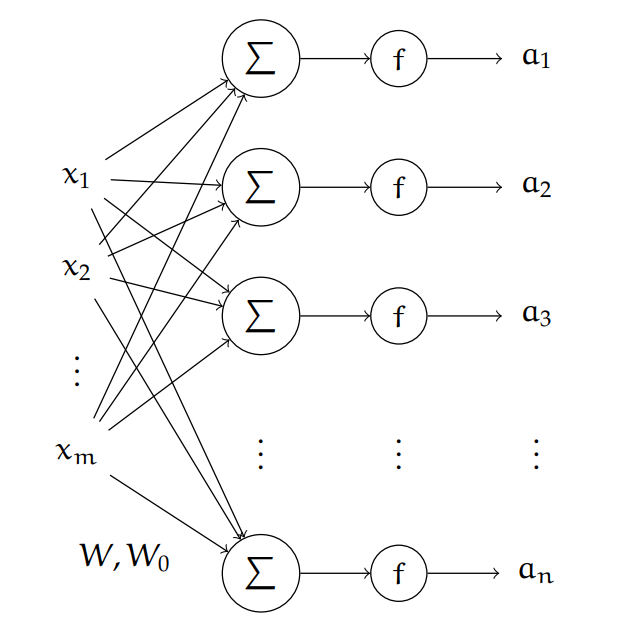
\includegraphics[scale=0.3]{Figures/ml_2.png}
    % \caption{Caption}
    \label{fig:my_label}
\end{figure}
Since each unit layer has a vector of weights and a single offset, we can consider the weights of
the whole layer as a matrix, W, and the collection of all the offsets as a vector $W_0$. If we
have m inputs, n units, and n outputs, then,
\begin{itemize}
    \item  W is an m $\times$ n matrix
     \item $W_0$ is an n$\times$  1 column vector,
     \item X, the input, is an m $\times$  1 column vector,
     \item Z = W$^T$X + $W_0$, the pre-activation, is an n$\times$  1 column vector,
\end{itemize}
and the output vector will be\\
\begin{equation*}
    A = f(Z) = f(W^Tx +W_0)
\end{equation*}

\subsubsection{Many layers}

A single neural network generally consists of multiple layers, where the output of the previous layer feeds as input to the next layer..\\
 We will use l to name a layer and 
let $m^l$ be the  number of inputs to the layer and $n^l$ be the number of outputs from the layer. Then, $W^l$ and $W^l _0$ are of shape $m^l \times n^l$, respectively. Let $f^l$ be the activation
function of layer  $ \ell$ . Then, the pre-activation outputs are the $n^l \times$ 1 vector, such that,
\begin{equation*}
    Z^l = {W^l}^T A^{l-1} + W_0^l
\end{equation*}
and the activation function outputs are simply the $n^l \times 1$ vector
\begin{equation*}
    A^l = f^l(Z^l)
\end{equation*}
We will use this structural diagram to organize our algorithmic thinking and implementation different parameters in deep neural network.
\begin{figure}[H]
    \centering
    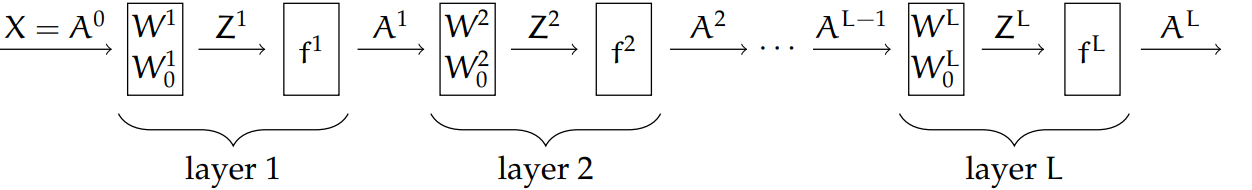
\includegraphics[scale=0.3]{Figures/ml__3.png}
    % \caption{Caption}
    \label{fig:my_label}
\end{figure}

As we saw here how a model of neural network function, the training and output from any model depends on the type of non linear functions Z, i.e. activation function we use in between the layers. Now, the question arises, how many types of activation functions are there?, and how we choose which one will be suitable for our model? We will addresses all these issues over the next section.

\subsection{ Activation function}
\label{subsection:Activationfunction}
There are three types of neural networks activation functions:
\subsubsection{Binary Step Function}
Binary step function depends on a threshold value which decides whether a neuron should be activated or not. This can be represented using the equation \autoref{eq:2}

\begin{equation} \label{eq:2}
   f(x) =  \begin{cases} 
      0 for x < 0 \\
      1 for x \geq 0 
   \end{cases}
\end{equation}
The output of the equation can be represented graphically as,
\begin{figure}[H]
    \centering
    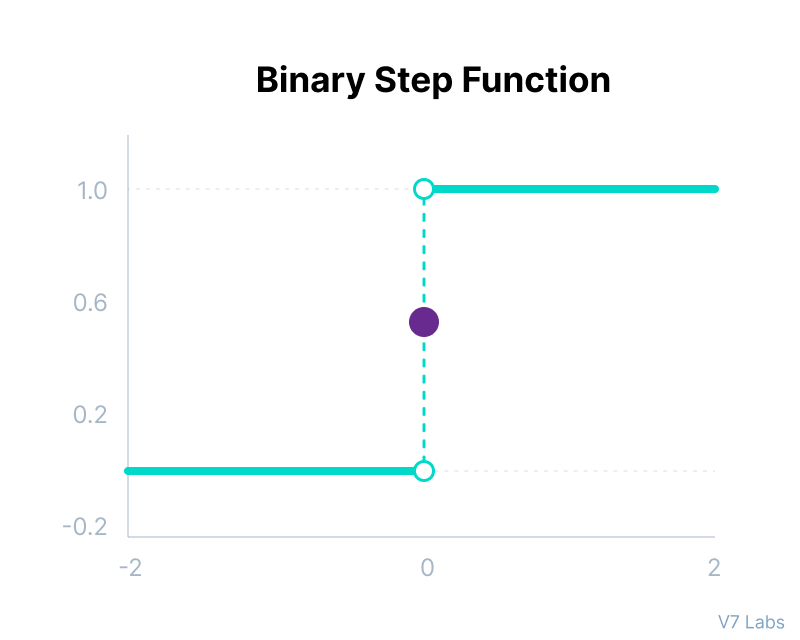
\includegraphics[scale=0.2]{Act_1.jpg}
    % \caption{Caption}
    \label{fig:my_label}
\end{figure}
The binary activation function is not always useful; a few of its limitations are:
\begin{itemize}
    \item We cannot use this activation function to provide us an output of multiclass problems, as it has only two labels of output.
    \item The gradient of the step function is zero, which causes a restriction in the back propagation process.
\end{itemize}

 
\subsubsection{Linear Activation Function}
Also known as identity Function, i.e. it can be represented using equation, and fig. below,
\begin{equation}
    f(x) = x
\end{equation}

\begin{figure}[H]
    \centering
    \includegraphics[scale=0.2]{Act_2.jpg}
    % \caption{Caption}
    \label{fig:my_label_02wwe}
\end{figure}

However, a linear activation function also has these two major problems :

\begin{itemize}
    \item It’s impossible to use back propagation as the gradient of the function is always a constant and has no relation with the input x.
    \item After use of linear activation function, without having dependence on a number of layers, the last layer will still be a linear function of the first layer. A linear activation function turns the neural network model into just one layer, which leads to model collapse.
\end{itemize}

 
\subsubsection{Non-Linear Activation Functions}

Non-linear activation functions solve the above limitations possessed by both linear activation functions and binary activation function as the derivative are possible and also related to the inputs, thus backpropogation are allowed here.

Few non-linear activation functions are:-\\
\textbf{Sigmoid / Logistic Activation Function}\\
Input is any real value(i.e. x $\in$ $\mathbb{R}$)and outputs $\in$ [0,1].\\
Mathematically, it can be represented as:\\
\begin{equation}
    f(x) = \frac{1}{1+e^{-x}}
\end{equation}
The output of the above equation is,
\begin{figure}[H]
    \centering
    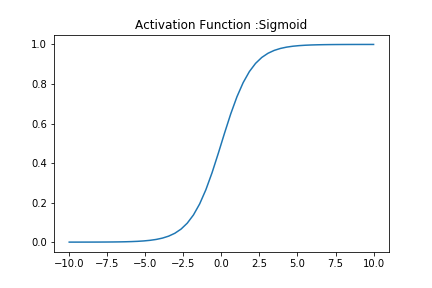
\includegraphics{Figures/sigmoid.png}
    % \caption{Caption}
    \label{fig:my_label}
\end{figure}

\textbf{Tanh Function}\\
Tanh function is very similar to the sigmoid/logistic activation function, with only difference in the output range of -1 to 1. 
Mathematically, it can be represented as;
\begin{equation}
    f(x) = \frac{e^x - e^{-x}}{e^x + e^{-x}}
\end{equation}
And, graphically, it can be represented as,\\
\begin{figure}[H]
    \centering
    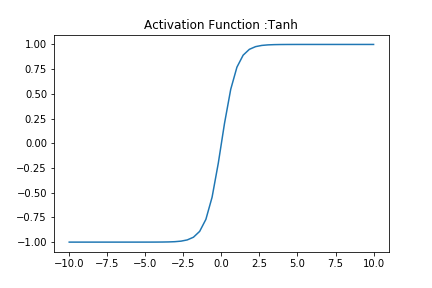
\includegraphics{Figures/Tanh.png}
    % \caption{Caption}
    \label{fig:my_label}
\end{figure}


Tanh activation function gives advantages as the output of the tanh activation function is Zero centered; thus, we can easily map the output values as strongly negative, neutral, or strongly positive. Another advantage is that the value of the hidden layers in a neural network has its values  between -1 to 1, and the mean for the hidden layer comes out to be 0 or very close to it. Therefore, it helps in centering the data and makes learning for the next layer much easier.

\textbf{ReLU} \\
ReLU stands for Rectified Linear Unit. ReLU has a derivative function, despite seems like linear function. It allows backpropagation and also simultaneously making it computationally efficient. The ReLU function does not activate all the neurons at the same time. The neurons get deactivated when its output is less than 0, that is,
\begin{equation}
    f(x) = max(0,x) = \begin{cases} 
      0 & z < 0 \\
      z & otherwise 
   \end{cases}
\end{equation}

\begin{figure}[H]
    \centering
    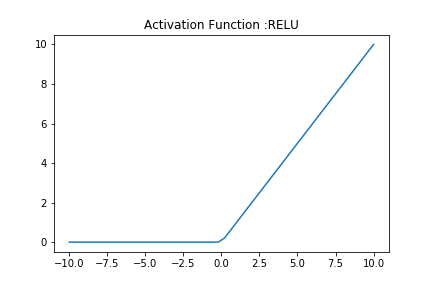
\includegraphics{Figures/RELU.png}
    % \caption{Caption}
    \label{fig:my_label}
\end{figure}


It is the most commonly used activation  function due to following unique features. Since ReLU activation function activate only a certain number of neurons, and it help them to do computation efficiently  in comparison to the sigmoid and tanh functions. The ReLU activation function also increase or decrease the rate of convergence towards global minimum of the loss function due to its linear, non saturating property[\cite{21}].

\textbf{Softmax}\\
It is used to calculate the relative probabilities. Like sigmoid activation function, the SoftMax function also returns the probability of each class. \\
It is the most commonly used activation function for the last or output layer of the neural network in the case of multi-class classification. \\
Mathematically it can be represented as:
\begin{equation}
    softmax(z_i) = \frac{exp(z_i)}{\sum_j exp(z_j)}
\end{equation}
\begin{figure}[H]
    \centering
    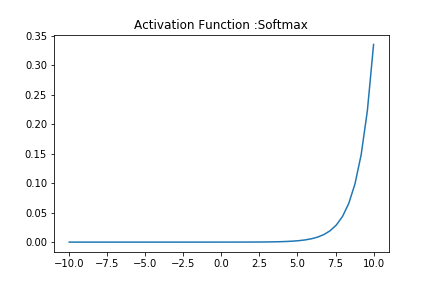
\includegraphics{Figures/softmax.png}
    % \caption{Caption}
    \label{fig:my_label}
\end{figure}
Here, we saw a few common activation functions, but how we can choose activation function for the given problem? 

\subsubsection{How to choose activation function for Hidden Layers}
The choice of activation function in between the layers depends on the type of problem we have, as it is summarized in the tree below.
 \begin{center}
    \begin{forest}
      [
      Network type?
       [Multilayer Perceptron
        [ReLU \\ Activation]
       ]
       [Convolutional Neural Net
        [ReLU \\ Activation]
         ]
        
       [Recurrent Neural Net
       [sigmoid Activation]
       [Tanh Activation]
       ]
      ] 
    %   [Multi-class\\ cross-Entropy \\Loss \\ Functions
    %   [Multi-class\\ Cross-Entropy\\ Loss]
    %   [Sparse Multiclass \\cross-Entropy \\loss]
    %   [Kullback\\ Leibler\\ Divergence \\Loss]
    %   ]
      
    \end{forest}
 \end{center}



\subsubsection{How to choose activation function for output layers}
% \begin{figure}[H]
%     \centering
%     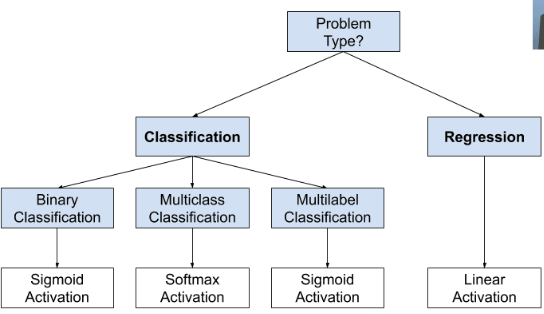
\includegraphics[scale=0.5]{Figures/ml__4.png}
%     % \caption{Caption}
%     \label{fig:my_label}
% \end{figure}
The activation function used in the final layer of the neural network depends on what type of output we need and on the type of prediction problem that we are solving, which can be summarized from the tree below.
\begin{itemize}
    \item \textbf{Regression}: one node, Linear Activation
    \item \textbf{Binary Classification}:one node per class, Softmax Activation
    \item \textbf{Multiclass Classification}:One node per class, softmax activation
    \item \textbf{Multilabel Classification}: One node per class, sigmoid activation
\end{itemize}

 \begin{center}
    \begin{forest}
      [
      Problem type?
       [Classification
        [Binary \\ Classification
         [Sigmoid Activation]
        ] 
        [Multiclass \\ Classification
         [Softmax Activation]
         ]
        [Multilabel \\ Classification
        [Sigmoid Activation]
        ]
       ]
       [Regression
       [Linear Activation]
       ]
    %   [Multi-class\\ cross-Entropy \\Loss \\ Functions
    %   [Multi-class\\ Cross-Entropy\\ Loss]
    %   [Sparse Multiclass \\cross-Entropy \\loss]
    %   [Kullback\\ Leibler\\ Divergence \\Loss]
    %   ]
      ]
    \end{forest}
 \end{center}

% \begin{figure}
%     \centering
%     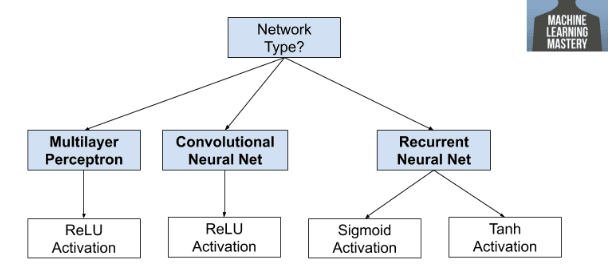
\includegraphics[scale=0.5]{Figures/ml__5.png}
%     % \caption{Caption}
%     \label{fig:my_label}
% \end{figure}















% Source
% \url{https://machinelearningmastery.com/choose-an-activation-function-for-deep-learning/}
% \url{https://www.v7labs.com/blog/neural-networks-activation-functions}
% ReLUs are especially common in internal (“hidden”) layers, and sigmoid activations are
% common for the output for binary classification and softmax for multi-class classification.(\url{https://openlearninglibrary.mit.edu/assets/courseware/v1/9c36c444e5df10eef7ce4d052e4a2ed1/asset-v1:MITx+6.036+1T2019+type@asset+block/notes_chapter_Neural_Networks.pdf}
\section{Training of Neural Network}



\subsection{Error backpropagation}
We will train our neural networks using gradient descent methods. It’s possible to use batch gradient descent, in which we sum up the gradient over all the points or stochastic gradient descent (SGD), where we take a small step with respect to the gradient after considering a single point at a time[\cite{23}].
% \textbf{Include theorem from} \url{https://openlearninglibrary.mit.edu/assets/courseware/v1/d81d9ec0bd142738b069ce601382fdb7/asset-v1:MITx+6.036+1T2019+type@asset+block/notes_chapter_Gradient_Descent.pdf}\\

we will always compute the gradient of the loss function with respect
to the weights for a particular value of (x, y). That tells us how much change is needed in the
weights, in order to reduce the loss experienced on this particular training. Let us understand with this example.\\
First, let’s us calculate and observe how the loss depends on the weights in the final layer, $W^L$ remembering
that our output is $A^L$, and using the shorthand loss to stand for Loss((f(x; W), y) which
is equal to Loss($A^L$, y), and finally that $A^L$ = $f^L$($Z^L$) and $Z^L$ = ${W^L}^T$ $A^{L-1}$, we can apply the chain  rule as:
\begin{figure}[H]
    \centering
    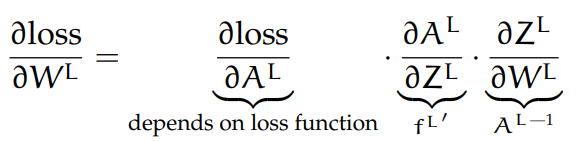
\includegraphics[scale = 0.3]{Figures/ml__6.png}
    % \caption{Caption}
    \label{fig:my_label}
\end{figure}
Here, we need to be little careful with the dimensions, and here we can note that it is true for any $ \ell$, including $ \ell$ = L\\
\begin{figure}[H]
    \centering
    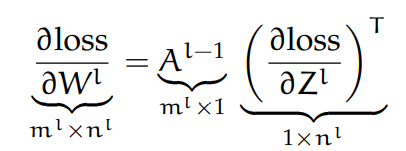
\includegraphics[scale=0.3]{Figures/ml__7.png}
    % \caption{Caption}
    % \label{fig:my_label}
\end{figure}
If we can repeatedly apply the chain rule, we will obtain this expression for the gradient of the loss with respect to the pre-activation function in the first layer:
\begin{figure}[H]
    \centering
    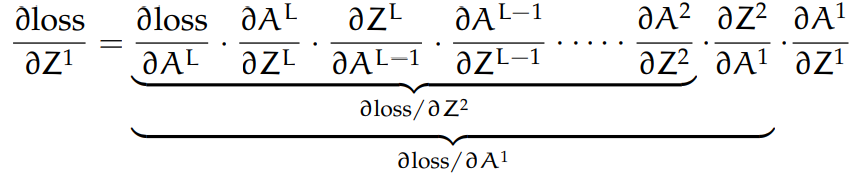
\includegraphics[scale=0.3]{Figures/ml__8.png}
    % \caption{Caption}
    \label{fig:my_label}
\end{figure}


Here,
\begin{itemize}
    \item $\frac{\partial loss}{\partial A^L}$ is $n^L \times 1$ and depends on the particular loss function you are using.
    \item $\frac{\partial Z^l}{\partial A^{l-1}}$ is $m^L \times n^L$ and is just $W^l$
    \item $\frac{\partial A^l}{\partial Z^l}$ is $n^L \times n^L$. Each element $\alpha_i ^l = f^l(z_i ^l)$. This means that $\frac{\partial \alpha_i ^l}{\partial z_j ^l}$ = 0 whenever i$\neq$ j. So, the off-diagonal elements of $\frac{\partial A^l}{\partial Z^l}$ are all 0, and the diagonal elements are $\frac{\partial \alpha_i ^l}{\partial z_j ^l}$= ${f^l}^'(z_j ^l)$
\end{itemize}
We can write the above equation as,
\begin{figure}[H]
    \centering
    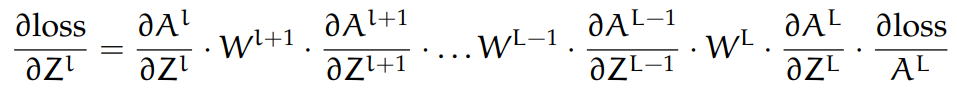
\includegraphics[scale=0.3]{Figures/ml__09.png}
    % \caption{Caption}
    \label{fig:my_label}
\end{figure}

This general process is called error back-propagation. The general idea is that we will do a forward
pass to compute all the $\alpha$ and z values at all the layers. Then, we can start work backward direction and compute the gradient of the loss with respect
to the weights in every layer, starting at last layer L and going back to layer 1, in this way model can update its weight, as can be shown below,\\
\begin{figure}[H]
    \centering
    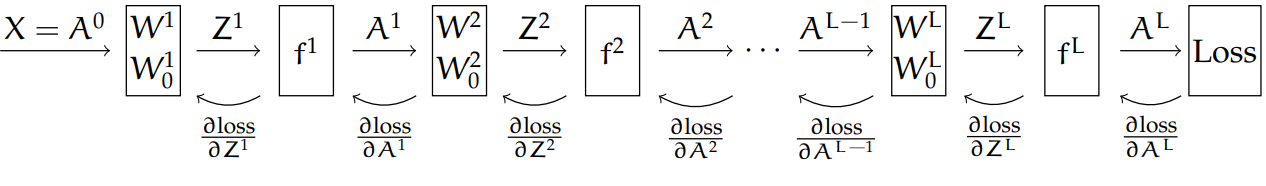
\includegraphics[scale=0.3]{Figures/ml__10.png}
    % \caption{Caption}
    \label{fig:my_label}
\end{figure}




Now, How we can do stochastic gradient descent training on a feed-forward neural network. This is the pseudo code to apply stochastic gradient descent,

% \begin{algorithm}
% \caption{\textit{SGD-NEURAL-NET(D_n,T, L, ($m^1$, ...$m^L$), ($f^1$,......,$f^L$))}}\label{alg:cap}
% \begin{algorithmic}
% \for {l=1 to L}
% \State $W_{ij} ^l ~ Gaussian(0, \frac{1}{m^l})$
% % \ $y = x^n$
% % \State $y \gets 1$
% % \State $X \gets x$
% % \State $N \gets n$
% % \While{$N \neq 0$}
% % \If{$N$ is even}
% %     \State $X \gets X \times X$
% %     \State $N \gets \frac{N}{2}$  \Comment{This is a comment}
% % \ElsIf{$N$ is odd}
% %     \State $y \gets y \times X$
% %     \State $N \gets N - 1$
% % \EndIf
% % \EndWhile
% \end{algorithmic}
% \end{algorithm}

\begin{lstlisting}[language=Python]
def SGD(f, theta0, alpha, num_iters):
    """
      Arguments:
      f -- the function to optimize, it takes a single argument
            and yield two outputs, a cost and the gradient
            with respect to the arguments
      theta0 -- the initial point to start SGD from
      num_iters -- total iterations to run SGD for
      Return:
      theta -- the parameter value after SGD finishes
    """
    start_iter = 0
    theta = theta0
    for iter in xrange(start_iter + 1, num_iters + 1):
        _, grad = f(theta)
  
        # there is NO dot product ! return theta
        theta = theta - (alpha * grad)
\end{lstlisting}



\section{Loss functions }
Now, the choice of a loss function for a particular problem is a very tedious task. We can take a rough idea about the loss function from this tree,\\
\resizebox{\linewidth}{!}{%
 \begin{center}
    \begin{forest}
      [
      Loss Function
       [Regression \\Loss\\ functions
        [Mean \\ Squared \\Error loss]
        [Mean\\ Squared \\Logarithmic \\Error loss]
        [Mean\\ absolute\\ Error\\ Loss]
       ]
       [Binary \\Classification\\ Loss \\Functions
       [Binary \\Cross- Entropy]
       [Hinge\\ Loss]
       [Squared\\ Hinge Loss]
       ]
       [Multi-class\\ cross-Entropy \\Loss \\ Functions
       [Multi-class\\ Cross-Entropy\\ Loss]
       [Sparse Multiclass \\cross-Entropy \\loss]
       [Kullback\\ Leibler\\ Divergence \\Loss]
       ]
      ]
    \end{forest}
 \end{center}
}

Like activation function, loss function also take different assumptions about the range of inputs it will take depending on the type of problem in hand. While designing the model of neural network, it become important to make things to fit well together. As, in particular, we will think about matching loss function with activation function of the last layer, $f^L$. This hypothesis can be infer from the table below, \autoref{tab:my_label_12}.\\
\begin{table}[h]
    \centering
    \begin{tabular}{ccc} \hline
   \textit{   Loss }  & \textit{ $f^L$} & \textit{Comments}\\ \hline
      squared   &  Linear &  --\\
      hinge  &  Linear &  for "maximum-margin" classification\\
      NLL &   Sigmoid &   negative log likelihood loss. Useful to \\ 
      &    &       train classification problem with C classes.\\
      NLLM & softmax & -- \\
      
    \end{tabular}
    \caption{Few loss functions corresponding to the last layer/ output layer activation function. There are many different types of the loss function following the kind of problem, whether it belongs to classification or regressions. }
    \label{tab:my_label_12}
\end{table}
There are also other loss function we have used to make our model better, such as "BinaryCrossentropy", "CategoricalCrossentropy", and
"SparseCategoricalCrossentropy" belonging to probabilistic losses. Also, "mean\_squared\_error", "mean\_absolute\_error", and "MeanSquaredError" belonging to regression losses.
 
\subsubsection{Two-class classification and log likelihood}

% For classification, the natural loss function is 0-1 loss, but we have already discussed the
% fact that it’s very inconvenient for gradient-based learning because its derivative is discontinuous. \\
For binary classification problems, which are useful in separation of signal and background, Hinge loss gives us another way, to make a smoother objective, penalizing the margins of the labeled points relative to the separator. The hinge loss is defined to be
\begin{equation*}
    L_h(guess, actual) = max(1-guess.actual,0)
\end{equation*}
when actual $\in$ \{+1, -1\}
 Using hinge loss, together with a squarednorm regularizer, forces the learning process to try and find a separator that has the
maximum margin relative to the data set. This optimization set-up is called a \textbf{support vector machine}. It was popular because it has a quadratic form that makes SVM to get easily optimized.

\subsubsection{Multi-class classification and log likelihood}
Multi-class classification with total of K classes, where the training label is represented with the one-hot vector $y = [y_1,...., y_k]^T$, where $y_k$= 1 if the example is of class k.Assume that our network uses softmax as the activation function (Which is most commomly used activation function for multi classification) in the last layer, so that the output is
$\alpha = [\alpha_1,....,\alpha_k]^T$, which represents a probability
distribution over the K possible classes. Then, the probability that our network predicts
the correct class for this example is $\Pi_{k=1} ^N \alpha_k ^y$ and the log of the probability that it is correct is $\sum_{k=1} ^k y_k \log \alpha_k$,so
\begin{equation*}
    L(guess, actual) = - \sum_{k=1} ^K actual_k.log(guess_k)
\end{equation*}





\section{Optimizing neural network parameters}
As neural networks consists of many parameters, our ultimate goal to minimize the loss function. The optimization can be done with help of standard gradient-descent softwares, but here, we can take advantages of the structure of the loss functions to improve optimization. The structure of loss function as a sum over terms, one training data point, help us to consider stochastic gradient methods. In this section, we will try to consider some alternative strategies for organizing training, and also to make easier to handle the step-size parameter.\\


\subsection{Batches}

Lets us assume we have an objective function of the form\\
\begin{equation*}
    J(W) = \sum_{i=1} ^n L(h(x^{(i)};W),y^{(i)})
\end{equation*}
where h is the function computed by a neural network, and W stands for all the weight
matrices and vectors in the network.\\
When we perform batch gradient descent, we use the update rule \\
\begin{equation*}
    W := W-\eta \nabla_W J(W), 
\end{equation*}
which is equivalent to 
\begin{equation*}
     W := W-\eta \nabla_W \sum_{i=1} ^n L(h(x^{(i)};W),y^{(i)})
\end{equation*}
Thefore, we add up the gradient of loss after each training point, with respect to W, and then take a step in the negative direction of the gradient to minimize the loss.\\


A more effective strategy for optimization is to take “average” between batch and stochastic gradient descent by using mini-batches. For a mini-batch of size k, we select k distinct data points uniformly at random from the data set and do the weight update based just on their contributions to the gradient.
\begin{equation*}
    W \leftarrow W-\eta \nabla_W \sum_{i=1} ^n L(h(x^{(i)};W),y^{(i)})
\end{equation*}
Most neural network software packages are set up to do mini-batches\cite{25}.\\

To select k unique data points at random from a large dataset is computationally difficult. An alternative strategy, if we have an efficient procedure for randomly shuffling the data set (or randomly shuffling a list of indices into the data set) is to operate
in a loop, roughly as follows:\\
\begin{algorithm}
\caption{\textit{MINI-BATCH-SGD(NN, data, k)}}\label{alg:cap}
\begin{algorithmic}
\State $n = length(data)$
\While{not done:}
     \State $RANDOM-SHUFFLE(data)$
     \For {i=1 to $\frac{n}{k}$}
           \State $BATCH-GRADIENT-UPDATE(NN,data[(i-1)k:ik])$
% \Require $n \geq 0$
% \Ensure $y = x^n$
% \State $y \gets 1$
% \State $X \gets x$
% \State $N \gets n$
% \While{$N \neq 0$}
% \If{$N$ is even}
%     \State $X \gets X \times X$
%     \State $N \gets \frac{N}{2}$  \Comment{This is a comment}
% \ElsIf{$N$ is odd}
%     \State $y \gets y \times X$
%     \State $N \gets N - 1$
% \EndIf
% \EndWhile
\end{algorithmic}
\end{algorithm}
then, we can easily divide the dataset into k mini batches.

\subsection{ Adaptive stepsize}

Picking the value for $\eta$ is difficult and time-consuming. As our networks become deep (with increase in the numbers of layers) we can find that magnitude of the gradient of the loss with respect the weights in the last layer,$\frac{\partial loss}{\partial W_L}$,may have significant differences from the gradient of the loss with respect to the weights in the first layer $\frac{\partial loss}{\partial W_1}$.\\

The output gradient is further multiplied by all the weight matrices of the network and is “fed
back” through all the derivatives of the activation functions. This can lead to a general problem
of \textbf{exploding or vanishing gradients}, in which the back-propagated gradient is either too big
or small.

\subsubsection{Running averages}


It is a computation strategy for estimating a weighted average for a sequence of data. Let us take data sequence be $\alpha_1, \alpha_2,......;$ then we define a sequence of running average values, $A_0, A_1, A_2,....$ using the equations
\begin{equation*}
      A_0 = 0
\end{equation*}
\begin{equation*}
         A_t = \gamma_t A_{t-1} + (1-\gamma_t)\alpha_t
\end{equation*}
where $\gamma_t$ $\in$ (0,1). If $\gamma_t$ is a constant, then this is a moving average, in which
\begin{equation*}
         A_T = \gamma A_{T-1} + (1-\gamma)\alpha_T
\end{equation*}
\begin{equation*}
       = \gamma(\gamma A_{T-2} +(1-\gamma)\alpha_{T-1}) +(1-\gamma)\alpha_T
\end{equation*}
\begin{equation*}
     = \sum_{t=0} ^T \gamma^{T-t}(1-\gamma)\alpha_t
\end{equation*}
So, you can see that inputs $\alpha_t$ closer to the end of the sequence have more effect on $A_t$ than early inputs.\\


\subsubsection{Momentum}
 we can use this method a bit like running averages to describe strategies for computing $\eta$. The simplest method is momentum, in which we try to “average” recent gradient updates so that if they have been bouncing oscillating in some direction, then we at least take out that component of the motion. For momentum, we have\\
\begin{equation*}
      V_0 = 0
\end{equation*}
\begin{equation*}
         V_t = \gamma V_{t-1} + \eta \nabla_W J (W_{t-1})
\end{equation*}
\begin{equation*}
         W_t =  W_{t-1} - V_t
\end{equation*}
This does not look like an adaptive step-size method. But, if we let
$\eta = \eta'(1-\gamma)$ then the rule looks exactly like doing an update with step size $\eta'$ on a moving average of the gradients with parameter $\gamma$:
\begin{equation*}
    M_0 = 0
\end{equation*}
\begin{equation*}
           M_t = \gamma M_{t-1} + (1-\gamma) \nabla_W J (W_{t-1})
\end{equation*}
\begin{equation*}
         W_t =  W_{t-1} - \eta'M_t
\end{equation*}

\begin{figure}[H]
    \centering
    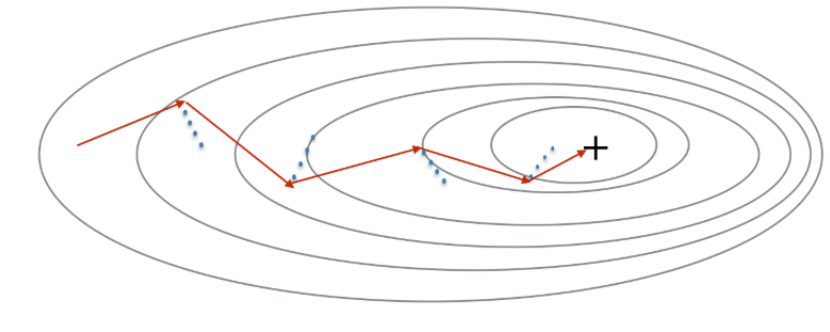
\includegraphics[scale=0.3]{Figures/ml__11.png}
    \caption{The red arrows show the change in the value of weight after one step of mini-batch gradient descent with use of momentum. The blue points show about the direction of the gradient with respect to
the mini-batch at each step. The Momentum smooths the path taken towards the local
minimum and further leads to faster convergence.\cite{21},\cite{25}}
    \label{fig:my_label}
\end{figure}

\subsubsection{Adadelta}
Here the idea is to take larger steps in parts of the space where J(W) get nearly flat (as there are no risks of taking too larger step due to the gradient being large) and smaller steps when it is steep. We’ll apply this idea to each weight, and at the end we obtain a method called adadelta. 
Even, here our weight are indexed by layers including input and output unit, just let $W_j$ be any weight in the network\\
\begin{equation*}
    g_{t,j} = \nabla_W J (W_{t-1})_j
\end{equation*}
\begin{equation*}
       G_{t,j }= \gamma G_{t-1, j} + (1-\gamma) g_{t,j}^2
\end{equation*}
\begin{equation*}
    W_{t,j} = W_{t-1,j}- \frac{\eta}{\sqrt{G_{t,j}+\epsilon}}g_{t,j}
\end{equation*}
% The sequence $G_{t,j}$ is a moving average of the square of the jth component of the gradient.
% We square it in order to be insensitive to the sign—we want to know whether the magnitude is big or small. Then, we perform a gradient update to weight j, but divide the step
% size by $\sqrt{G_{t,j}+\epsilon}$,which is larger when the surface is steeper in direction j at point $W_{t-1}$ in weight space; this means that the step size will be smaller when it’s steep and larger when
% it’s flat.

\subsubsection{Adam}

Adam has become the most common and default method of managing step sizes neural networks. The moving averages of the gradient
and squared gradient, which estimates the mean and variance of the gradient for weight j:
\begin{equation*}
     g_{t,j} = \nabla_W J (W_{t-1})_j
\end{equation*}
\begin{equation*}
        m_{t,j} = B_1 m_{t-1,j} + (1-B_1) g_{t,j}
\end{equation*}
\begin{equation*}
        v_{t,j} = B_2 v_{t-1,j} + (1-B_2) g_{t,j}^2
\end{equation*}

If we initialize $m_0$ = $v_0$ = 0, then there will always be bias(slightly too small). So we will correct the bias by defining,
\begin{equation*}
    \hat{m}_{t,j} = \frac{m_{t,j}}{1-B_1^t}
\end{equation*}
\begin{equation*}
    \hat{v}_{t,j} = \frac{v_{t,j}}{1-B_2^t}
\end{equation*}
\begin{equation*}
    W_{t,j} = W_{t-1, j} - \frac{\eta}{\sqrt{ \hat{v}_{t,j}+\epsilon}}\hat{m}_{t,j} 
\end{equation*}
Adam did not have a huge effect on the result after making small changes in the model, which makes it an efficient method.

\section{Regularization}

Till now, we have only discussed how we can optimize loss on our training data. As discussed before, the risk of overfitting is still persistent. This overfitting problem can be rectified with the help of increasing our data size, which is the case nowadays where the deep neural network uses large data size. Nonetheless, there are several strategies for regularizing a neural network, and sometimes they can be important. This can be done using the implementation of early stopping, where the idea is train on the training set, and on every epochs, (pass through the whole training set, or possibly more frequently), evaluate the loss of the current W on a validation set. Here, it is observed that the loss on the training set goes down fairly consistently with each number of iteration, and the loss on the validation set will initially decrease, but then begin to increase
again. Once we observe that the validation loss is systematically increasing, we can stop training the model and return the weights that had the lowest validation error.\\

Another simple method is to penalize the norm of all the weights,This method is known as weight decay,
\begin{equation*}
    J(W) = \sum_{i=1}^n Loss(NN(x^{(i)}), y^{(i)};W) + \lambda ||W||^2
\end{equation*}
we end up with an update of the form\\
\begin{equation*}
    W_t = W_{t-1}(1-\lambda_\eta) - \eta (\nabla_W Loss(NN(x^{(i)}), y^{(i)};W_{t-1}))
\end{equation*}

This rule has the form of first “decaying” $W_{t-1}$ by a factor of (1 -$\lambda \eta$) and then taking a gradient step.\\
Other few methods are:-

% \subsection{Methods related to ridge regression}
% Early stopping is the easiest to implement and is in fairly common use. The idea is
% to train on your training set, but at every epoch (pass through the whole training set, or
% possibly more frequently), evaluate the loss of the current W on a validation set. It will
% generally be the case that the loss on the training set goes down fairly consistently with
% each iteration, the loss on the validation set will initially decrease, but then begin to increase
% again. Once you see that the validation loss is systematically increasing, you can stop
% training and return the weights that had the lowest validation error.\\
% Another common strategy is to simply penalize the norm of all the weights,This method is known as weight decay, because when we take the gradient of the objective
% \begin{equation*}
%     J(W) = \sum_{i=1}^n Loss(NN(x^{(i)}), y^{(i)};W) + \lambda ||W||^2
% \end{equation*}
% we end up with an update of the form\\
% \begin{equation*}
%     W_t = W_{t-1}(1-\lambda_\eta) - \eta (\nabla_W Loss(NN(x^{(i)}), y^{(i)};W_{t-1}))
% \end{equation*}

% This rule has the form of first “decaying” $W_{t-1}$ by a factor of (1 -$\lambda \eta$) and then taking a gradient step.


\subsection{Dropout}

The contains a simple idea, it suggest rather than perturbing the data every time we train, we will make changes in the
network. Here, we will randomly, from each dataset, after selecting a unit layer prohibit them from participating  in the training. Therefore, all of the units will have to take a 
kind of overall responsibility for getting the answer right, and will not be able to rely
on any small subset of the weights to do all the necessary computation. This tends also to
make the network more robust to data perturbations.\\
When we are done training and want to use the network to make predictions, we multiply all weights by p to achieve the same average activation levels. In the forward pass during training, we let\\
\begin{equation}
    \alpha^l = f(z^l) * d^l
\end{equation}
where * denotes component-wise product and $d^l$ is a vector of 0’s and 1’s drawn randomly
with probability p. The backwards pass depends on $\alpha^l$ so we do not need to make any
further changes to the algorithm.
Another modern alternative method to dropout, is batch normalization.\\
\subsection{Batch Normalization}

Here, idea is when training is done with mini-batches, the idea is to standardize the input values for each mini-batch, subtracting off the mean and dividing by the standard deviation of each input dimension. This gives us similar effect to adding noise and dropout. Each mini-batch of data ends up getting mildly perturbed, which prevents the network from exploiting very particular values of the data points.\\
% So, when training with mini-batches, the idea is to standardize the input values for each mini-batch, subtracting off the mean and dividing by the standard deviation of each input dimension. This Batch normalization ends up having a regularizing effect for similar reasons that adding noise and dropout do: each mini-batch of data ends up being mildly perturbed, which prevents the network from exploiting very particular values of the data points.\\


\section{ROC Curve}
Another metric tom measure the output is the Receiver Operating Characteristic (ROC) curve output after training, defined with respect to
a given class \textit{C}. Given a point x and model that outputs a P(C|x) probability that x belongs to the class C. Given T , a threshold, x belongs to C if and only if P(C|x) $\geq$ T . If T = 1, a point is labeled as belonging to class, C only if the model is 100\% sure. If T = 0, every point is labeled as belonging to the class C\\
Each value of the threshold T generates a point (False Positive, True Positive) and, then, the ROC curve is the curve formed by going through T = 0 to T = 1. A good model will have a curve that increases quickly from 0 to 1, the different ROC curve depending over output can be seen in \autoref{fig:my_label-2}
\begin{figure}[H]
    \centering
    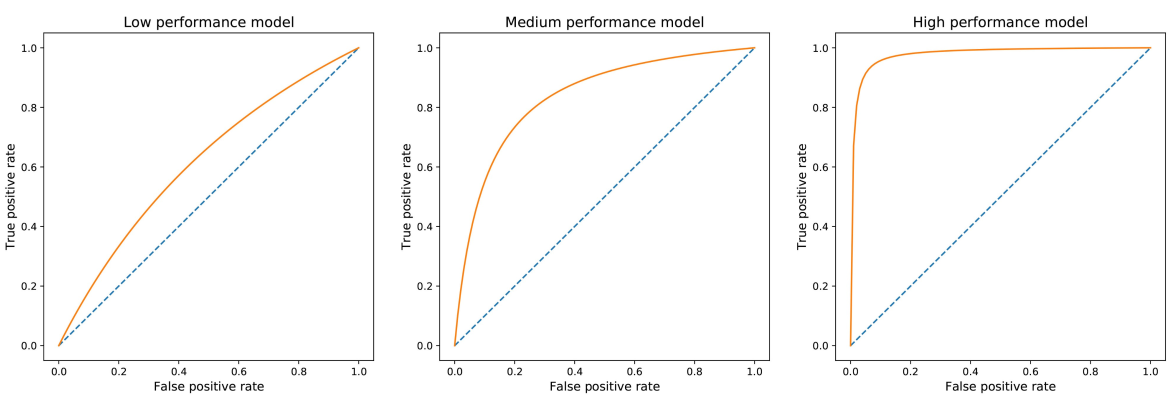
\includegraphics[scale=0.3]{13__ml.png}
    \caption{ROC curves depending on the effectiveness of the model}
    \label{fig:my_label-2}
\end{figure}











%     \textbf{(Maths part may be excluded)}



% 1. \url{https://openlearninglibrary.mit.edu/assets/courseware/v1/9c36c444e5df10eef7ce4d052e4a2ed1/asset-v1:MITx+6.036+1T2019+type@asset+block/notes_chapter_Neural_Networks.pdf}

% \url{https://www.mygreatlearning.com/blog/types-of-neural-networks/}
% \url{MIT lecturre from where you have learnt}






























































































\setcounter{equation}{0}
\setcounter{table}{0}
\setcounter{figure}{0}
%\baselineskip 24pt

\chapter{\label{d}Signal and Background}
What are signal and background? The signal corresponds to the features, process, or whatever events we are interested in studying. This signal could correspond to the production of a Higgs, or maybe of a pair of W bosons, or maybe it just corresponds to events with two high energy jets or events in them. While the backgrounds are the events that may seem like signals but we are not interested in.\\
We took s simulated sample of the resonance particles of the top quark; Tprime, and other t-quark particle such as $\Bar{t}tH$, thq, and ttgg for the training and testing of the deep neural network model.
The associated production of top quarks with the Higgs boson, either in pairs ($\Bar{t}tH$) or singly (tH), provides direct experimental access to the top-Higgs
coupling. The $\Bar{t}tH (tH)$ production mode, while proceeding at a rate of about 100(1000) times smaller than gluon fusion, bears a highly distinctive experimental signature, which includes leptons and/or jets from the decay of the two (single) top quarks as shown in \autoref{fig:my_label_tth}. \\
With the increase of the LHC energy from 8 to 13 TeV for Run 2, the ttH production cross section is expected to increase by a factor four. However, such process still remains rare, and searches for ttH production have been driven by the higher sensitivity achieved in Higgs decay modes with larger branching fractions.[\cite{14}] \\
\begin{figure}[H]
    \centering
    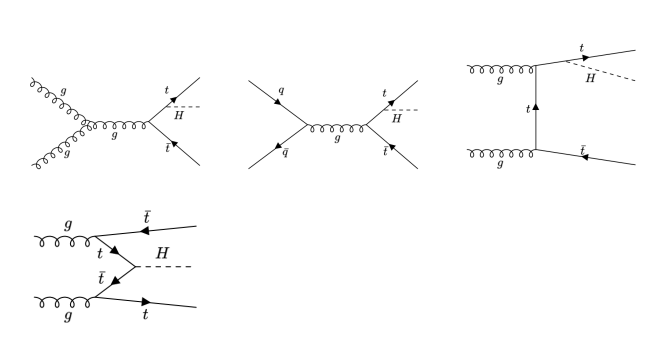
\includegraphics[scale=0.7]{tth_1.png}
    \caption{Feynman diagrams depicting $t\Bar{t}H$ production modes}
    \label{fig:my_label_tth}
\end{figure}


As the standard model(SM) is complete as a low-energy effective theory describing all known fundamental particles and their interactions. But there are also a few problems that SM cannot explain. There are various theories of new physics beyond the SM that predict the additional particles that can affect the quantum corrections to the Higgs boson mass and answer question, which is known as "hierarchy problem". One of the proposed promising new states is vector-like quarks.\cite{12}

Vector-like quarks (VLQs) are hypothetical spin-1/2 coloured particles, labeled $T^'$ and $B’$, with electric charges of +2e/3 and -1e/3, respectively. Their left-handed and right-handed components transform in the same way under the Standard Model gauge group. A vector-like top quark partner T' has two production modes. One is pair production through the strong interaction while the other is single production mode through the electroweak interaction\cite{12}. The T' quark could couple to bW, tZ, or tH, resulting in the corresponding T' quark decays as shown with Feynman diagram in the \autoref{fig:my_label_T'}. We will use this VLQ as the signal.\\




\begin{figure}[H]
    \centering
    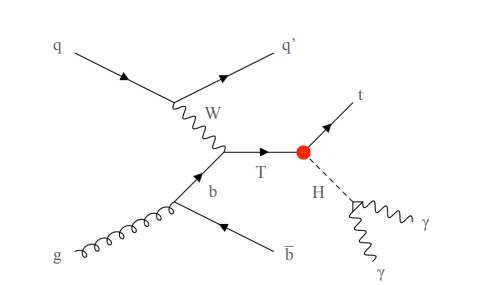
\includegraphics[scale=0.5]{T'.png}
    \caption{Leading-order Feynman diagram for single T’ production}
    \label{fig:my_label_T'}
\end{figure}





For the another two ntuples of thq and ttgg, the Feynman diagrams are plotted in the  \autoref{fig:my_label_ttgg}, \autoref{fig:my_label_ttgg_12}, and \autoref{fig:my_label_thq}  respectively.

\begin{figure}[H]
    \centering
    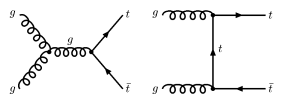
\includegraphics[scale=0.5]{ttgg.png}
    \caption{ttgg Feynman diagram}
    \label{fig:my_label_ttgg}
\end{figure}

\begin{figure}[H]
    \centering
    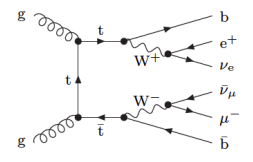
\includegraphics[scale=0.5]{ttgg__.png}
    \caption{Feynman diagram for ttgg}
    \label{fig:my_label_ttgg_12}
\end{figure}




\begin{figure}[H]
    \centering
    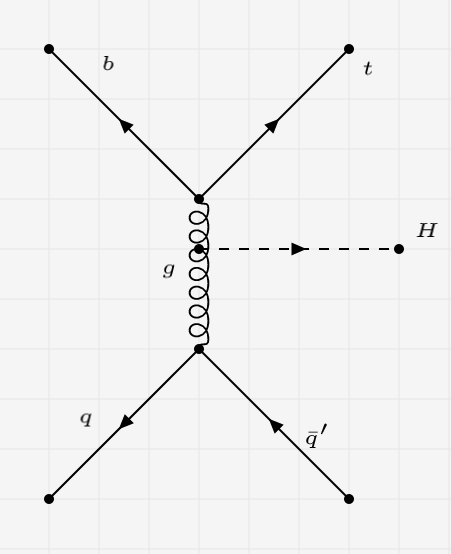
\includegraphics[scale =0.5]{thq.png}
    \caption{Feynman diagram of thq}
    \label{fig:my_label_thq}
\end{figure}




Few of the plots of variables of these simulated samples are shown below,
\begin{figure}[H]
\begin{subfigure}{.5\textwidth}
  \centering
  % include first image
  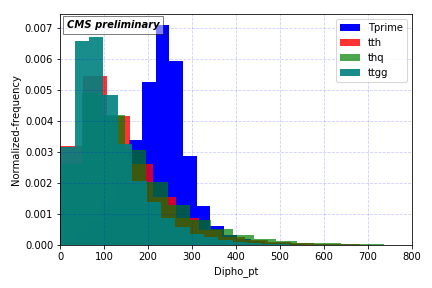
\includegraphics[width=.8\linewidth]{Inputs/variable_Dipho_pt.png}  
  \caption{}
  \label{fig:sub-first}
\end{subfigure}
\begin{subfigure}{.5\textwidth}
  \centering
  % include second image
  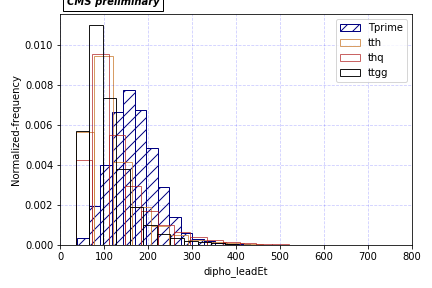
\includegraphics[width=.8\linewidth]{Inputs/variable_Dipho_leadEta.png}  
  \caption{}
  \label{fig:sub-second}
\end{subfigure}



\begin{subfigure}{.5\textwidth}
  \centering
  % include third image
  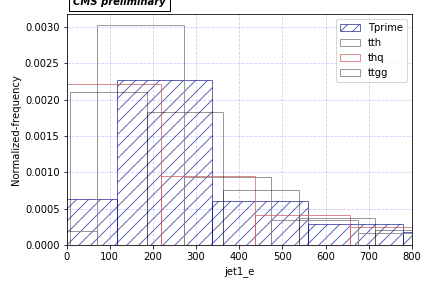
\includegraphics[width=.8\linewidth]{Inputs/variable_jet1_e.png}  
  \caption{}
  \label{fig:sub-third}
\end{subfigure}
\begin{subfigure}{.5\textwidth}
  \centering
  % include fourth image
  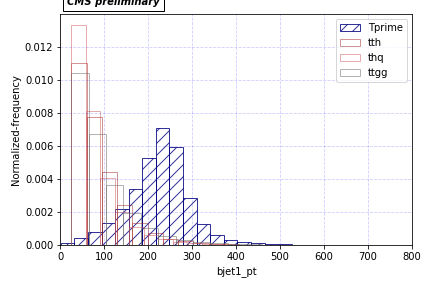
\includegraphics[width=.8\linewidth]{Inputs/variable_bjet1_pt.png}  
  \caption{}
  \label{fig:sub-fourth}
\end{subfigure}


\begin{subfigure}{.5\textwidth}
  \centering
  % include third image
  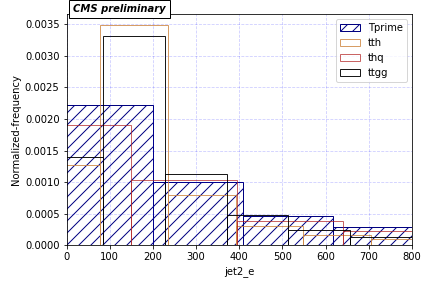
\includegraphics[width=.8\linewidth]{Inputs/jet2_e.png}  
  \caption{}
  \label{fig:sub-fifth}
\end{subfigure}
\begin{subfigure}{.5\textwidth}
  \centering
  % include fourth image
  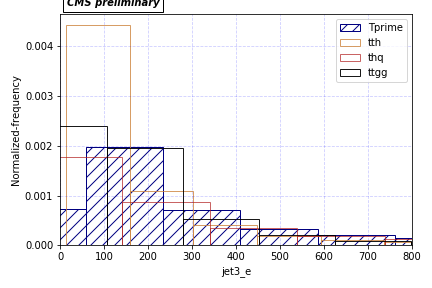
\includegraphics[width=.8\linewidth]{Inputs/jet3_e.png}  
  \caption{}
  \label{fig:sub-fourth}
\end{subfigure}

\begin{subfigure}{.5\textwidth}
  \centering
  % include third image
  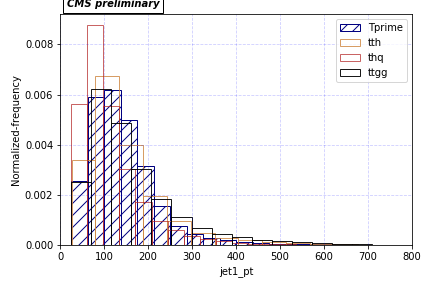
\includegraphics[width=.8\linewidth]{Inputs/jet1_pt.png}  
  \caption{}
  \label{fig:sub-third}
\end{subfigure}
% \begin{subfigure}{.5\textwidth}
%   \centering
%   % include fourth image
%   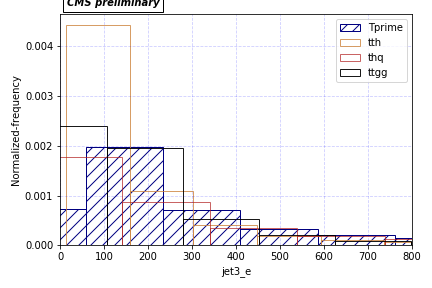
\includegraphics[width=.8\linewidth]{Inputs/jet3_e.png}  
%   \caption{}
%   \label{fig:sub-fourth}
% \end{subfigure}
\caption{Simulated sample plot for different variables, for each figure plotted above the signal is Tprime and the background is tth, thq, and ttgg. From top to bottom, plots for different variable are as, (a) Plot for $Dipho\_P_T$, (b) Plot for $Dipho\_leadEt$, (c)Plot for $jet1\_e$, (d) Plot for $bjet1\_P_T$, (e) Plot for $jet2\_e$, (f) Plot for $jet3\_e$, and (g) Plot for $jet1\_P_T$ }
\label{fig:fig}
\end{figure}
 
In the given \autoref{fig:fig}, we plotted a representation for a few variables. from this figure, we can see how our signal (Tprime) cannot get clearly separated from our background( $tt\gamma \gamma$, $\Bar{t}th$, and thq. Our main motivation is to make a better separation of the Tprime, signal in this case from the backgrounds i.e., $tt\gamma\gamma$, $\Bar{t}th$, and thq.








% Questions needed to be addressed?
% \begin{itemize}
%     \item What are signal and background?
%     \item 
% \end{itemize}































% About Simulated sample 
%     \begin{itemize}
    
%         % \item Feynman Diagram(details about tth, ttgg, thq, Tprime)
%         \item Kinematics features, Kinematic variables definition and its derivations(about all of the variables and their meaning)
%         \item 
%         \item What feature of (suppose $Dipho_PT$) you are measuring.
%         % \item What is Tprime, tth, thq, ttgg? How these are formed
%         % \item how the varibale looks lie. Present a few of them
        
%     \end{itemize}
    
    

\setcounter{equation}{0}
\setcounter{table}{0}
\setcounter{figure}{0}
%\baselineskip 24pt


% %%%%%%%%%%%%%%%%%%%%%%QUESTIONS MAY GET FRAMED FROM HERE%%%%%%%%%%%%%%%%%%%%%%%%%%%%%%%%%%%%%%%%%%%%%%
% \begin{itemize}
%     \item Why we measure luminosity in $fb^{-1}$
% \end{itemize}
\chapter{\label{results}Results and Discussion}
In the previous section, from \autoref{fig:fig}, we observed that the separation of the signal and the background events for different datasets were not clearly visible. This is a basic problem of classifications. To separate and make a proper visualization of the events as signal or background; there are several machine learning methods used traditionally, such as Boosted Decision Trees(BDTs), XGBoosts, and many other TMVA based machine learning methods. To separate signal and background, python based  modules such as Keras, which is based on the high-level wrapper for the machine learning frameworks Theano (\url{www.deeplearning.net/software/theano/}) and TensorFlow (\url{www.tensorflow.org}), they were mainly used to set up deep neural networks.\cite{29} \cite{30}
[\url{http:// tmva.sourceforge.net}]



\section{Uses of DNN }
The Deep Neural network(DNN) \footnote{All the code related to this work can be found here: \url{https://github.com/raj2022/M.Sc.-thesis/tree/main/Codes}} has been applied for training over the ntuple of tth, thq, ttgg and Tprime. The dataset was converted into the array using modules root2numpy(\url{https://scikit-hep.org/root_numpy/}), and further randomize it using rec2array. By using Pandas DataFrame we converted the array and further feed it into the model after splitting them as train and test data sets. The basic working model of the neural network is shown in the \autoref{fig:my_label_5.1}.
\begin{figure}[H]
    \centering
    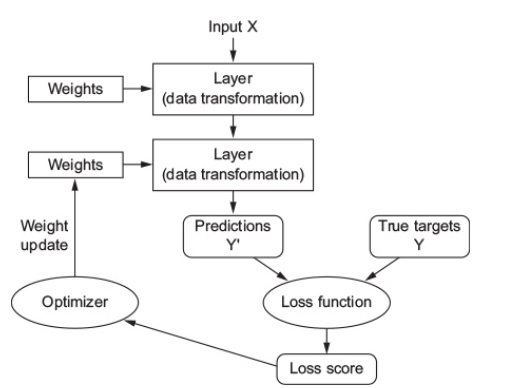
\includegraphics[scale=0.6]{Inputs/12__ml.png}
    \caption{Neural network scheme. Image source: [Chollet, 2017]}
    \label{fig:my_label_5.1}
\end{figure}

\section{DNN model}
Deep neural network (DNN) is used here for training the data and further testing the model. Keras module, Sequential used to make the DNN model. The basic architecture of our model are as follow, given in \autoref{tab:my_label_00}. Our model was made to train total 5,33,457 trainable parameters,and we also have total number of datasets around this number. The model was given total of 29 different input features( \autoref{tab:my_label_1}) in the first layer. To make neural layer more deep and to get a better training output, there were 4 extra hidden layers consisting of 200, 100, 100 and 100 nodes were added to the input layer. The output of successive layers goes as input to the next layer after passing through the  ReLU activation function(as shown in \autoref{fig:my_label_3}). For each layer, we have used dropout layer to save our model from collapsing.  For each 3 input model will drop a value, the model architecture is shown in the \autoref{fig:my_label_arch}.\\

For each input layers, we have provided weight or random state as 5, which will be getting updated after each training. The rationale behind choose these specific parameters such as the number of nodes, layers, epochs is to improve our training accuracy, and it was completely based on hit and trail method. \\

The output layer consist  only a single node for binary classification and again changed for multi classification, depending on the number of outputs we required as the outputs. In this semester project report, the output will only behave either as signal or as background. The  output layer also depend on whether the output required in binary or multiclass. For binary classification, the common activation function used is 'sigmoid', which we have already discussed in \autoref{subsection:Activationfunction} 
The model was compile with the binary cross entropy loss function \& categorical\_crossentropy loss function depending on the type of classifications. To avoid the model collapsing issues, we have used ADAM optimizer in the model and to prevent the training from over-fitting, the model is trained with accuracy matrices.\\

The model was fitted with the given dataset by splitting it into training and testing dataset in the ratio of 80:20, that is 80\% of the data used for training and 20\% of the data used for testing the model. The model has also provided with validation dataset, which is sample of dataset used to provide an unbiased evaluation of a model fit on training dataset while having model hyper-parameter(discussed in \autoref{tab:my_label_00}. Here the validation dataset are one-fourth of training data. This model was trained in the batch of 900, which means for every training, it would divide the dataset into 900 mini batches and run through all over the training data. The number of epochs of the model is 100, it employs the model has run through 100 times in total, after each run, model update or optimize its weight/ random\_state by itself  depending on the output of the error/loss and other hyper parameter. The model was further tested on the given testing dataset.  
   
   
 \begin{figure}[H]
     \centering
     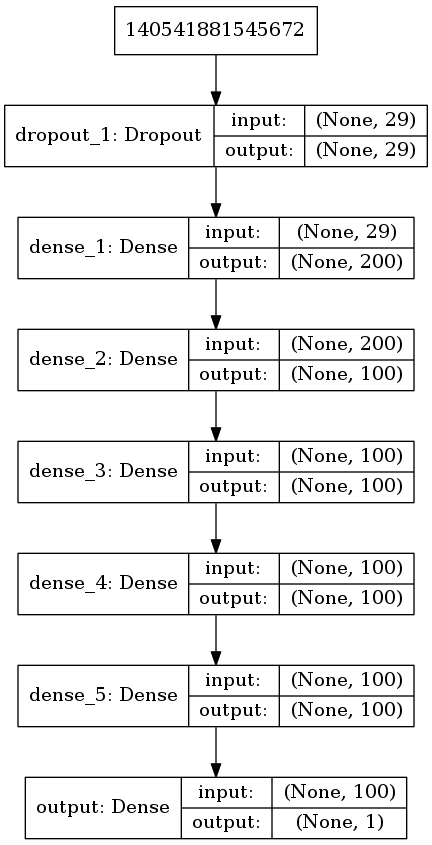
\includegraphics[scale=0.2]{TPrime_ttgg/clf_plot____.png}
     \caption{Basic architecture of our DNN Model }
     \label{fig:my_label_arch}
 \end{figure}
 %%%%%%%%%%%%%%%%%%Table Describing the model%%%%%%%%%%%%%%%%%%%%%%%%%%%%%%%%%%%%%%%%%%%%%%%%%%%%%%
 \begin{table}[H]
     \centering
     \begin{tabular}{|ccc|}\hline
       Options   &   & Description \\\hline
    Model      &    sequential  &   -   \\
    Number of Inputs      &    29  &    as given in \autoref{tab:my_label_1}  \\
    Number of layers (Input)     & 200     &  $Dense_1$    \\
        Hidden  &  200    &  $Dense_2$    \\
         Hidden &  100    &   $Dense_3$   \\
        Hidden  & 200     &  $Dense_4$    \\
        Hidden  & 200     & $Dense_5$     \\
        Output  & 1      &  $Dense_6$    \\
    Activation function(Hidden Layer)      &  ReLU    &   Same for both binary\\  
    & & classification and multiclassification   \\
      Activation layer(Output)    & sigmoid     &  For binary classification    \\
                                  &  Softmax  & For multi classification    \\
    Loss function   &   Binary cross entropy    & For binary classification \\
                    &    categorical\_crossentropy  & For multi classification \\
    Optimizer      &     ADAM     &     -\\
    Matrices     & Accuracy    &  \\
    BatchSize      & 900  & Batch size used for a single gradient  \\
                      &    &     step during training  \\
    NumEpochs      & 100 &   Number of training epochs \\
    Verbose &    1  &  Verbosity during training \\\hline
    
     \end{tabular}
     \caption{Configurations of the Keras model used for training and testing purposes}
     \label{tab:my_label_00}
 \end{table}
   
\section{Correlation between signal and background variable}
A correlation function represents a measurement between the strength of a linear relationship between two quantitative variables. There are two types of correlation, positive correlation and negative correlation. Positive correlation represents a relationship between two variables in which both variables move in the same direction. This means when one variable increases while the other also increases and vice versa While negative correlation is a relationship where one variable increases as the other decreases, and vice versa. A correlation of 1 or +1 shows a perfect positive correlation, which means both the variables move in the same direction. A correlation of -1 shows a perfect negative correlation, which means as one variable goes down, the other goes up \cite{27}. Here for the comparison of the variables (given in \autoref{tab:my_label_1}) from two different datasets were calculated using Pearson Correlation Coefficient Formula, which is,
\begin{equation}
    r = \frac{n(\sum xy)- \sum x \sum y}{\sqrt{[n \sum x^2 - (\sum x)^2][n \sum y^2 - (\sum y)^2]}}
\end{equation}
Where,\\
n = Quantity of Information \\
$\sum x$ = Total of the First Variable Value \\
$\sum y$ = Total of the Second Variable Value\\
$\sum xy$ = Sum of the Product of first \& Second Value\\
$\sum x^2$ = Sum of the Squares of the First Value\\
$\sum y^2$ = Sum of the Squares of the Second Value\\

The correlation plot for the given variables of Tprime and ttgg are plotted in the \autoref{fig:example_correlation}.
  \begin{figure}[H]
    \centering
    \subfloat[\centering Background(ttgg)]{{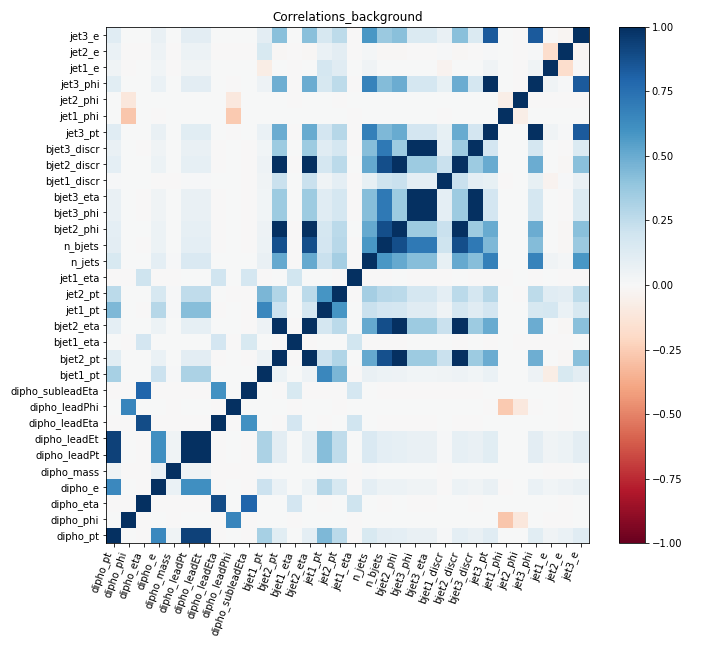
\includegraphics[width=10cm]{TPrime_ttgg/new_correlation_background.png} }}%
    \qquad
    \subfloat[\centering Signal(Tprime)]{{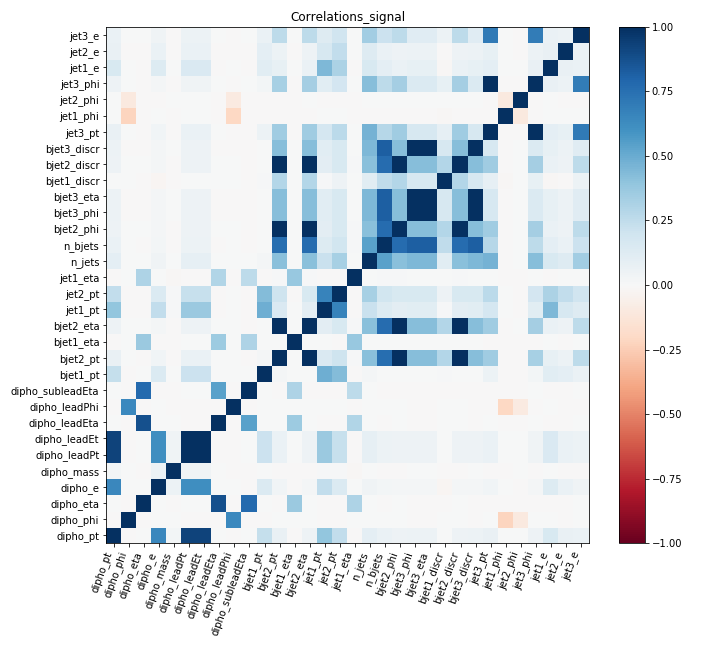
\includegraphics[width=10cm]{TPrime_ttgg/new_correlation_signal.png} }}%
    \caption{Correlation plot of two different datasets for different variables. Above, (a) Correlation plot for background(ttgg) and below, (b) Correlation plot for signal(Tprime)}
    \label{fig:example_correlation}
\end{figure}

   \begin{table}[h!]
    \centering
    \begin{tabular}{|c|c|}\hline
     Sl. No.    & Variables \\\hline
       1  & dipho\_pt \\
        2  & dipho\_phi \\
         3  & dipho\_eta \\
          4  & dipho\_mass \\
           5  & dipho\_leadPt \\
            6  & dipho\_leadEt \\
             7  & dipho\_leadEta \\
              8  & dipho\_leadPhi \\
               9  & dipho\_subleadEta \\
                10  & bjet1\_pt \\
                 11  & bjet2\_pt \\
                  12  & bjet1\_eta \\
                   13  & bjet2\_eta \\
                    14  & jet1\_pt \\
                     15  & jet2\_pt \\
                      16  & jet1\_eta \\
                       17  & n\_jets \i\
                        18  & n\_bjets \\
                         19  & bjet2\_phi \\
                          20  & bjet3\_phi \\
                        %   1  & bjet3_eta \\
                            21  & bjet1\_discr \\
                             22  & bjet2\_discr \\
                              23  & bjet3\_discr \\
                              24 & jet3\_pt \\
                                % & jet1\_phi \\
                                % & jet2\_phi \\
                              25  & jet3\_phi \\
                                26  & jet1\_e \\
                                  27  & jet2\_e \\
                                    28  & jet3\_e \\ 
                                    29 & dipho\_e \\\hline
           
    \end{tabular}
    \caption{Variables of $\Bar{t}th$, Tprime(T'), thq, and ttgg used in separation of signal and Background}
    \label{tab:my_label_1}
\end{table}
   
 \section{Binary Classifications}
 
Using the above discussed DNN model, when fitted with batch size of 900, provided random state is 5 and epochs is 100 on the training dataset of Tprime and ttgg. We will obtain the output of signal and background as shown in the figure \autoref{fig:my_label_DNN_output}. The training and testing done using the deep neural network can be verified using the model accuracy and loss. The model training and testing loss and accuracy comparison have been shown in the \autoref{fig:my_label_00}  and  \autoref{fig:my_label_accuracy_ttgg} \\
 
   
\begin{figure}[H]
    \centering
    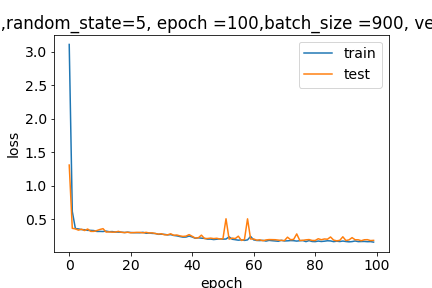
\includegraphics[scale=0.6]{TPrime_ttgg/loss_TPrime_ttgg.png}
    \caption{Training and testing loss when Tprime is used as signal and ttgg as the \\background}    \label{fig:my_label_00}
\end{figure}
%%%%%%%accuracy%%%%%%%%%%%%%
\begin{figure}[H]
    \centering
    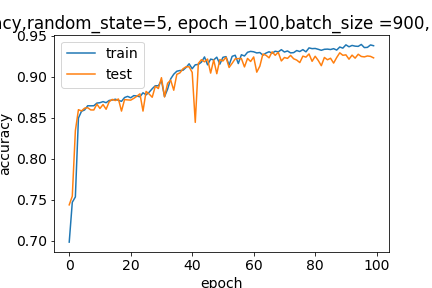
\includegraphics[scale=0.5]{TPrime_ttgg/accuracy_TPrime_ttgg.png}
    \caption{Training and testing model accuracy when Tprime is used as signal and ttgg as the background}
    \label{fig:my_label_accuracy_ttgg}
\end{figure}

%  The model output after training for signal and background separation are plotted in the fig. 5.7.  In this figure, our signal is plotted over 1 and rest background goes to zero.
 \begin{figure}[H]
     \centering
     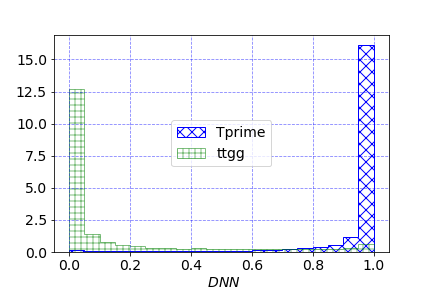
\includegraphics[scale=1]{TPrime_ttgg/output_TPrime_ttgg.png}
     \caption{Output of training using the DNN(Deep Neural Network). Here signal(Tprime) and background(ttgg) are clearly separated with background as 0 and signal corresponds to 1. }
     \label{fig:my_label_DNN_output}
 \end{figure}
 
 The performance analysis of the DNN model can be done with the help of the Receiving operator Characteristic(ROC) Curve plot for both the training and testing samples. The output ROC curve are plotted in the \autoref{fig:my_label_ROC_ttgg}
\begin{figure}[H]
    \centering
    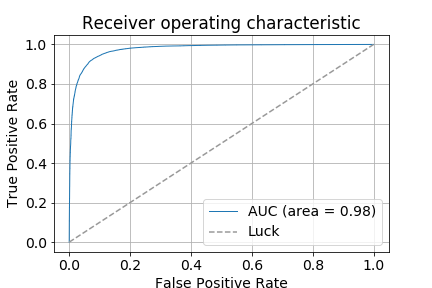
\includegraphics[scale=0.7]{ROC_curve_TPrime_ttgg.png}
    \caption{ROC curve for the training out of Tprime as signal and ttgg as the background}
    \label{fig:my_label_ROC_ttgg}
\end{figure}
%%%%%%%

For the comparison of the models, we can consider any other model of machine learning. Let's take infamous Boosted Decison Tree (BDT) model, it is used very frequently for data training at LHC. 
The BDT which can also distinguish between signal like and background like events. The output from this model of BDT classifier is plotted in \autoref{fig:my_label_BDT}. The area under the ROC Curve is 0.8863, while the training and testing output is around 82\% and 83 \% respectively. The input dataset for training and testing was T' and ttgg. The dataset was splitted over 33\% for the testing and 67\% for training. 


\begin{figure}[H]
    \centering
    \includegraphics[scale=0.7]{adaboost_classifier.png}
    \caption{Boosted Decision Tree(BDT), ROC curve  }
    \label{fig:my_label_BDT}
\end{figure}


 %%%%%%%%%%%%%%%%%
 
 Further, the model is used to train and test for the different combinations with the datasets. All the output scores of these training and testing are summarized in the \autoref{tab:my_label_0021}. The output plot for training with Tprime as signal and $\Bar{t}th$ \& ttgg as background plotted in \autoref{fig:my_label_000}. In this figure, we can see the Tprime (signal) corresponds to 1 (plotted in blue) while $\Bar{t}th$ \& ttgg as background corresponds to 0.
  
  \begin{figure}[H]
     \centering
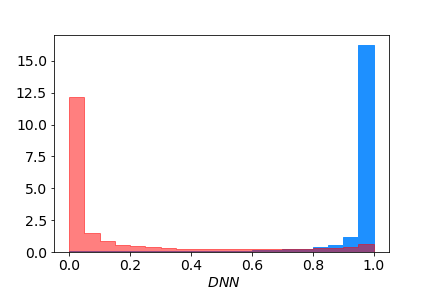
\includegraphics[scale=1]{TPrime_ttgg&tth&thq/output_TPrime_ttgg_&tth.png}
     \caption{Output of training from the DNN(Deep Neural Network). Here signal(Tprime) and background(ttgg  \& $\Bar{t}th$ ) are clearly separated with background as 0 and signal corresponds to 1. }
     \label{fig:my_label_000}
 \end{figure}
 
 
 With the combination of all the three datasets as the background (ttgg  \& $\Bar{t}th$ \& thq), and the Tprime as signal, we plotted the results. The ROC-curve for this setup is plotted in the \autoref{fig:my_label_89}, and the model accuracy \& loss are plotted in \autoref{fig:my_label_23} and \autoref{fig:my_label_009} respectively.
 
\begin{figure}[H]
    \centering
    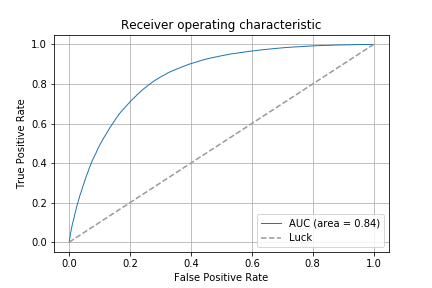
\includegraphics[scale=0.7]{TPrime_ttgg&tth&thq/ROC_curve_TPrime_ttgg_&tth&thq.png}
    \caption{ROC curve for the training output of Tprime as signal and ttgg, tth, and thq as the background}
    \label{fig:my_label_89}
\end{figure}

\begin{figure}[H]
    \centering
    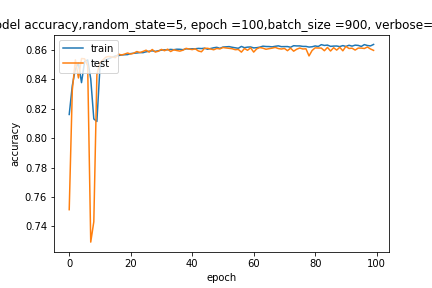
\includegraphics[scale=0.5]{TPrime_ttgg&tth&thq/model_accuracy_TPrime_ttgg_&tth&thq.png}
    \caption{Training and testing model accuracy when Tprime is used as signal and ttgg, tth, and thq were used as the background. To train different dataset over a single dataset are known as multi-class classification. }
    \label{fig:my_label_23}
\end{figure}

\begin{figure}[H]
    \centering
    \includegraphics[scale=0.6]{TPrime_ttgg&tth&thq/loss_TPrime_ttgg_&tth&thq.png}
    \caption{Training and testing loss when Tprime is used as signal and ttgg, tth, and thq were used as the background. To train different dataset over a single dataset are known as multi-class classification. }
    \label{fig:my_label_009}
\end{figure}


%  \section{TPrime and ttgg}
%  \begin{figure}[H]
%     \centering
%     \subfloat[\centering label 1]{{\includegraphics[width=5cm]{TPrime_ttgg/loss_TPrime_ttgg.png} }}%
%     \qquad
%     \subfloat[\centering label 2]{{\includegraphics[width=5cm]{TPrime_ttgg/accuracy_TPrime_ttgg.png} }}%
%     \caption{2 Figures side by side}%
%     \label{fig:example}%
% \end{figure}

%  \begin{figure}[H]
%      \centering
%      \includegraphics[scale=0.2]{TPrime_ttgg/clf_plot____.png}
%      \caption{Caption}
%      \label{fig:my_label}
%  \end{figure}
 
%  \begin{figure}[H]
%      \centering
%      \includegraphics[scale=0.5]{TPrime_ttgg/loss_TPrime_ttgg.png}
%      \caption{Caption}
%      \label{fig:my_label}
%  \end{figure}

%   \begin{figure}[H]
%      \centering
%      \includegraphics[scale=0.5]{TPrime_ttgg/new_correlation_background.png}
%      \caption{Caption}
%      \label{fig:my_label}
%  \end{figure}
 
 
%   \begin{figure}[H]
%      \centering
%      \includegraphics[scale=0.5]{TPrime_ttgg/new_correlation_signal.png}
%      \caption{Caption}
%      \label{fig:my_label}
%  \end{figure}
 


%  \begin{figure}[]
%      \centering
%      \includegraphics[scale=0.5]{TPrime_ttgg/accuracy_TPrime_ttgg.png}
%      \caption{Caption}
%      \label{fig:my_label}
%  \end{figure}
% \subsection{Correlation between signal and background variable}

\begin{table}[H]
    \centering
     \caption{Table with training and testing accuracy \%}
    \begin{tabular}{|c|c|c|c|}\hline
        Signal & Background & Training Accuracy(\%) & Testing Accuracy(\%) \\\hline
        TPrime & ttgg & 93.30 & 92.06  \\
        TPrime & ttgg\& tth & 89.84 & 89.07\\
        TPrime & ttgg\& tth\& thq & 86.36 & 86.10 \\ \hline
    \end{tabular}
    \label{tab:my_label_0021}
\end{table}

If we compare out DNN outputs for each process combination from the \autoref{tab:my_label_0021}, and also by comparing \autoref{fig:my_label_DNN_output} \& \autoref{fig:my_label_000}, we find that the training and testing accuracy are decreasing. To rectify these issues, we plan to implement multi-class classification, which we will be discussing this in the next section.
%%%%%%%%%%%%%%%%%%%%%%%%%%%%%%%%%%%%%%%%%%%%%%%%
%%%%%%%%%%%%%%%%%%%%%%%%%%%%%%%%%%
\section{Multi class Classification}
For the case of multi-class classification, we cannot use the same model of binary classifications(\autoref{tab:my_label_00}). We tried to create a different model, to avoid the frequent case of model collapsing, the model summary can be seen from \autoref{fig:multicalss} we try to use batch normalization and dropout layers after each dense layers. \dots 

\begin{wrapfigure}{l}{0.5\textwidth}
\centering
\includegraphics[width=.98\linewidth]{Inputs/clf_plot_multiclass___.png}
\caption{mode summary for the multi class classifications}
\label{fig:multicalss}
\end{wrapfigure}
% \lipsum[1]
The model obtains the same input variable, as the previous model for the binary classifications \autoref{fig:my_label_arch}. The  total number of input variables are 29 as given in \autoref{tab:my_label_1}. It is a general technique that can be used to normalize the inputs to a layer. We use first layer of batch normalization and divides the layers into mini batches. The output of this layer goes as input of the subsequent layer and we again use batch normalization and this continues till the output layer.The Output layer consists of 4 different outputs as we were dividing it into 4 different classes of Tprime($T^'$), $\Bar{t}th$, thq, and tt$\gamma \gamma$, respectively. \\
Deep neural networks(DNN) are sometimes very challenging to train, not least because the input from prior layers can change after weight update. Thus, by addition of batch normalization, it can be used to normalize the inputs given to a layer. The batch regularization accelerated the training rate and in some cases by halving the epochs or better. and further provides some regularization (two regularization, L1 and L2), and further reducing the generalization error.\\
The activation function used for inner layers were "ReLU", while the activation function for the output layer were "softmax". The corresponding loss function for multicalss training were "categorical\_crossentropy" with "ADAM" optimizer.

The training output of this model is plotted in the \autoref{fig:my_label_0099211} for accuracy and \autoref{fig:my_label-098365}, for model loss.


% \begin{figure}[htbp]
%   \raggedright
%     \includegraphics[scale=0.4]{Inputs/clf_plot_multiclass___.png}
%     \caption{Multiclass model summary}
%     \label{fig:my_label}
% \end{figure}


\begin{figure}[H]
    \centering
    \includegraphics[scale=0.7]{Model_accuracy_multiclass.png}
    \caption{Multiclass classification output for accuracy of training and testing}
    \label{fig:my_label_0099211}
\end{figure}


\begin{figure}[H]
    \centering
    \includegraphics[scale=0.7]{Model_loss_multiclass.png}
    \caption{Multiclass classification output for model loss of training and testing}
    \label{fig:my_label-098365}
\end{figure}
% \section{Mult-classification Outputs}
% Add the ROC curve 


% \setcounter{equation}{0}
% \setcounter{table}{0}
% \setcounter{figure}{0}
% %\baselineskip 24pt


    


% \subsection{Add following for better understanding}
% \begin{itemize}
%     \item Epoch change correpsonding to accuracy
% \end{itemize}



\chapter{\label{summary}Summary and Conclusions}\
In this report, we saw how we can use machine learning (Deep Neural Network) techniques to classify data from CMS, as the signal and background. We mainly focused on four simulated datasets, that was Tprime, $\Bar{t}th$, thq, and tt$\gamma \gamma$. In all of this dataset, only ttgg has non Higgs background. Here, the resonant particle, Tprime was the signal and rest, $\Bar{t}th$, thq, and tt$\gamma \gamma$ as the background. We also learn about deep learning techniques and its implementation. We also saw how deep neural networks (DNN) used to train and modify themselves to give a better optimized outputs. Usually, the output from this methods are better as compared to the other machine learning techniques used to separation, which is evident after the comparison of the output of two different model in \autoref{fig:my_label_BDT} for BDT and \autoref{fig:my_label_DNN_output} for the DNN output. The both training was done with the same dataset.\\

During the training through DNN, the output from the training of Tprime and ttgg was very good as expected with model accuracy of 93.30 \% for training and 92.06 \% for testing. ROC curve ouput is also excellent. This may be due to presence of non Higgs background, ttgg dataset as the background. When all the datasets were combined to the same DataFrame, the problem of model collapse was very feasible as also we can see from the output in \autoref{tab:my_label_0021}. The training and testing accuracy started to decrease. This model problem has been rectified with the use of multi classification training of the dataset instead of the binary classification. In multi classification each dataset will perform simultaneous training with the signal dataset simultaneously. As expected the model output are much improved compared to the previous binary classification model. The training and testing accuracy are 99.87\% and 99.86\% respectively. \\
The training over the model of multi classification can be done over any number of background. The expected resulted from this models are far better in comparison to Boosted Decision Tree(BDT), TMVA(DNN), etc\dots. As expected, we obtained a better classification output for multiclass compared to previous binary classification. Multiclass are a generalized way and less time consuming, whereas the binary classification are tedious and have to be done attentively.\\
The results of this report constitute an important development on how we can implement machine learning techniques for the search of few properties of new particles at the LHC. This result from the machine learning separation can be used to segregate the raw data from the CMS as signal and background and could be very efficient also.
% \newpage
% Address this questions:
% Why DNN, why not other?
% The Main Goal: To build a DNN to differentiate between signal and background events in an
% CMS data set
% %%%%%
% \begin{itemize}
%     \item How the signal efficiency and background efficiency are calculating?
    
% \end{itemize}

\setcounter{equation}{0}
\setcounter{table}{0}
\setcounter{figure}{0}
%\baselineskip 24pt


    






\begin{thebibliography}{9}

\begin{enumerate}
\item M. Konishi,Associated production of top quarks with the Higgs boson at $\sqrt{s}$ =13 TeV. Paper presented at XXV International Workshop on Deep-Inelastic Scattering and Related Subjects, 3-7 April 2017, University of Birmingham, UK 

\item ATLAS, CMS Collaboration, Measurements of the Higgs boson production and decay rates and constraints on its couplings from a combined ATLAS and CMS analysis of the LHC pp collision data at $\sqrt s$ = 7 and 8 TeV, JHEP 08 (2016) 045 [arxiv:1606.02266]
 
\item The CMS Collaboration, Machine learning technique for signal-background separation of nuclear interaction vertices in the CMS detector,CMS-DP-2020-036 ; CERN-CMS-DP-2020-036


\item D. Bourilkov,Machine and Deep Learning Applications in Particle Physics,
[arxiv:1912.08245], \url{https://arxiv.org/pdf/1912.08245.pdf}

\item Y. LeCun, Y. Bengio and G. Hinton, Nature 521, 436 (2015). doi:10.1038/nature14539


\item D., Frédéric ; Peters, Y.et al.Top Quark Physics at the Tevatron, \url{https://ui.adsabs.harvard.edu/abs/2013IJMPA..2830013D}

\item J Mora :Thesis, Deep learning applied in the classification of events generated at the ATLAS experiment, \url{https://hdl.handle.net/11673/49967}


\item Ngairangbam, V.S., Bhardwaj, A., Konar, P. et al. Invisible Higgs search through vector boson fusion: a deep learning approach. Eur. Phys. J. C 80, 1055 (2020). https://doi.org/10.1140/epjc/s10052-020-08629-w

\item  K. Albertsson et al., Machine learning in high energy physics community white paper. J. Phys. Conf. Ser. 1085(2), 022008 (2018)

\item A. Radovic, M. Williams, D. Rousseau, M. Kagan, D. Bonacorsi,
A. Himmel, A. Aurisano, K. Terao, T. Wongjirad, Machine learning at the energy and intensity frontiers of particle physics. Nature
560(7716), 41–48 (2018)

\item P. Baldi, K. Bauer, C. Eng, P. Sadowski, D. Whiteson, Jet substructure classification in high-energy physics with deep neural
networks. Phys. Rev. D 93(9), 094034 (2016)

\item CMS Draft Analysis Note:CMS AN-21-105, Search of a Vector Like Quark T' $\longrightarrow$ tH in diphoton final state. \url{https://prsaha.web.cern.ch/prsaha/Tprime_analysis/AN-21-105_temp.pdf}

\item He, K., Ren, S., Sun, J., \& Zhang, X.Deep Residual Learning for Image Recognition (2016), CoRR, abs/1512.03385

\item G. Krintiras, ttH and tH production at 13 TeV(2017), Conference Report,CMS CR -2017/176: \url{ https://cdsweb.cern.ch/record/2272651/files/CR2017_176.pdf}


\item \url{https://cms.cern/detector}
\item \url{https://cms.cern/detector/bending-particles}
\item \url{https://cms.cern/detector/bending-particles}
\item \url{https://cms.cern/news/how-cms-detects-particles}
\item \url{https://cms.cern/detector/identifying-tracks/silicon-strips}
\item \url{https://cms.cern/detector/computing-grid}
\item \url{https://machinelearningmastery.com/}
\item \url{https://keras.io/}
\item \url{https://towardsdatascience.com/}
\item \url{https://www.thomasgmccarthy.com/an-introduction-to-collider-physics-ix}
\item \url{https://openlearninglibrary.mit.edu/courses/course-v1:MITx+6.036+1T2019/courseware/Week7/neural_networks_2/}
\item \url{https://www.phys.ufl.edu/~avery/ivdgl/itr2001/proposal_all.pdf}
\item \url{https://edusera.org/machine-learning/}
\item \url{https://www.displayr.com/what-is-correlation/}

\item Guest D., Cranmer K.,Whiteson D., Deep Learning and Its Application to LHC Physics,Annu. Rev. Nucl. Part. Sci. 2018. \url{https://doi.org/10.1146/annurev-nucl101917-021019}


\item The CMS Collaboration, Machine learning technique for signal-background separation of nuclear interaction vertices in the CMS detector, CMS Performance Note(2020),CMS DP -2020/036
% \item G. Reuter, personal communication. [Must be accompanied with a letter of permission and must not be used to support a central claim, result, or conclusion.]
\end{enumerate}

\end{thebibliography}



















% %\clearpage
%\addcontentsline{toc}{chapter}{Appendices}
\begin{appendices}
\chapter{\label{appendix}(AUC-ROC Curve in Machine Learning)}
The AUC-ROC curve helps us visualize how well our machine learning classifier is performing.
\section{What is the AUC-ROC curve?}
The Receiver Operator Characteristic (ROC) curve is an evaluation metric for binary classification problems. It is a probability curve that plots the TPR against FPR at various threshold values and essentially separates the ‘signal’ from the ‘noise’. The Area Under the Curve (AUC) is the measure of the ability of a classifier to distinguish between classes and is used as a summary of the ROC curve.\\
The higher the AUC, the better the performance of the model at distinguishing between the positive and negative classes.\\
When AUC = 1, then the classifier is able to perfectly distinguish between all the Positive and the Negative class points correctly. If, however, the AUC had been 0, then the classifier would be predicting all Negatives as Positives, and all Positives as Negatives.\\
https://www.analyticsvidhya.com/blog/2020/06/auc-roc-curve-machine-learning/
\end{appendices}


\setcounter{equation}{0}
\setcounter{table}{0}
\setcounter{figure}{0}
%\baselineskip 24pt


    




% %\clearpage
%\addcontentsline{toc}{chapter}{Appendices}
\begin{appendices}
\chapter{\label{appendix}(CMS)}
\begin{figure}
    \centering
    \includegraphics[scale=0.1]{Figures/cms_detector.png}
    \caption{Source: \url{https://cms.cern/detector}}
    \label{fig:my_label_detect}
\end{figure}
\end{appendices}


\setcounter{equation}{0}
\setcounter{table}{0}
\setcounter{figure}{0}
%\baselineskip 24pt
% }
\end{document}
